% For long urls to break nicely and do not make overfull.
% Needed this line before documentclass
\RequirePackage[hyphens]{url}

\documentclass[11pt,a4paper,leqno,titlepage,twoside]{book}

%%%%%% packages %%%%%%%%%%
\usepackage{mystylearticle}
\usepackage{balance}
\usepackage{multicol} 
\usepackage{nonfloat}
\usepackage{enumitem}
\usepackage{wallpaper}
\usepackage{sectsty}
\usepackage{bbding}
\usepackage{pifont}
\usepackage{arydshln} % doted lines in tables
\usepackage{rotating} 
\usepackage[utf8]{inputenc} %para los acentos

%%%%%% fuente por defecto %%%%%%%%%%
\renewcommand{\familydefault}{\sfdefault}


%%%%%% figuras especiales %%%%%%%%%%
\newcommand\myfigure[1]{%
\bigskip\noindent\begin{minipage}{\linewidth}%{0.9\columnwidth}
\centering%
#1%
%figure,caption, and label go here
\end{minipage}\medskip}

%%%%%% nombres %%%%%%%%%%
\renewcommand{\contentsname}{Contenidos}
\renewcommand{\chaptername}{Cap\'\i tulo}
\renewcommand{\bibname}{Bibliograf\'\i a}
\renewcommand{\figurename}{Figura}
\renewcommand{\tablename}{Tabla}

%%%%%% pagina en blanco %%%%%%%%%%

\def\blankpage{%
      \clearpage%
      \thispagestyle{empty}%
      \addtocounter{page}{-1}%
      \null%
      \clearpage}


%%%%%% colores del tema %%%%%%%%%%
\definecolor{oyellow}{rgb}{1,0.835294117647059,0.133333333333333}
\definecolor{oblue}{rgb}{0.0352941176470588,0.450980392156863,0.541176470588235}
\definecolor{ogreen1}{rgb}{0.0196078431372549,0.650980392156863,0.576470588235294}
\definecolor{ogreen2}{rgb}{0.0588235294117647,0.737254901960784,0.568627450980392}
\definecolor{ored}{rgb}{0.929411764705882,0.258823529411765,0.215686274509804}

%%%%%% secciones con color %%%%%%%%%%
\chapterfont{\color{oblue}}
\sectionfont{\color{oblue}}
\subsectionfont{\color{ogreen1}}
\subsubsectionfont{\color{ogreen2}}


%%%%%% referencias con color %%%%%%%%%%
\hypersetup{colorlinks=true,
			linkcolor = oblue,
            urlcolor  = oblue,
            citecolor = oblue,
            anchorcolor = oblue}

%%%%%% bullets en itemize personalizados %%%%%%%%%%
\setlist[itemize,1]{label={\color{oblue}\ding{226}}} %\EllipseShadow
\setlist[itemize,2]{label={\color{oblue}\ding{227}}} %\EllipseSolid
\setlist[itemize,3]{label={\color{oblue}\ding{254}}} %\Ellipse

%%%%%% path graficos %%%%%%%%%%			
\graphicspath{{../pdf/}{C:/DATOS/MBIT/Proyecto/MBITProject_Data4all/Memoria/graphs/}}


%%%%%% headers and footers %%%%%%%%%%
\pagestyle{fancy}
\renewcommand{\sectionmark}[1]{\markright{\thesection\ #1}}
\fancyhf{}
% \fancyhead[LO]{\tt Versi\'on preliminar \today}
% \fancyhead[RE]{\tt Versi\'on preliminar \today}

\newcommand\PageBoxODD{
	\setlength{\fboxrule}{0cm}
	\fcolorbox{oyellow}{oyellow}{\begin{minipage}[t][0.75cm][c]{\textwidth}{\qquad\bf OCTOPUS} DATA INSIGHTS \hfill \thepage\qquad$ $\end{minipage}}}
	
\newcommand\PageBoxEVEN{
	\setlength{\fboxrule}{0cm}
	\fcolorbox{oyellow}{oyellow}{\begin{minipage}[t][0.75cm][c]{\textwidth}{\qquad\thepage\hfill\bf OCTOPUS} DATA INSIGHTS\qquad$ $\end{minipage}}}

\fancyfoot[CE]{\PageBoxEVEN}
\fancyfoot[CO]{\PageBoxODD}

\renewcommand{\headrulewidth}{0pt}
\renewcommand{\footrulewidth}{0pt}


\fancypagestyle{plain}{%
  \fancyhf{}%
  \renewcommand{\headrulewidth}{0pt}
  \fancyfoot[CE]{\PageBoxEVEN}
  \fancyfoot[CO]{\PageBoxODD}
}




% %%%%%%%%%%%%%%%%%%%%%%%%%%%%%%%% BEGIN DOCUMENT %%%%%%%%%%%%%%%%%%%%%%%%%%%%%%%%%%%%%%

\begin{document}


%%%%%% title page %%%%%%%%%%

\begin {titlepage}

% Cover picture
% \begin{pgfpicture}{0cm}{0cm}{\textwidth}{\textheight}
% \pgfputat{\pgfxy(-12,-4)}{\pgfbox[center,center]{\begin{picture}(0,0)(0,0)\resizebox{40cm}{30cm}
% {
\includegraphics{portada.jpg}}\end{picture}}}
% % Title and authors
% \pgfputat{\pgfxy(0,5)}{\pgfbox[left,center]{\Huge\textbf{AN\'ALISIS DE REDES SOCIALES}}}
% \pgfputat{\pgfxy(0,4)}{\pgfbox[left,center]{\Huge\textbf{PARA RECURSOS HUMANOS}}}
% \pgfputat{\pgfxy(0,2)}{\pgfbox[left,center]{\textbf{Fabio Inui\qquad Teresa Mart\'\i nez \qquad Javier Quintana \qquad Silvia Santos }}}
% % Versiones preliminares
% \pgfputat{\pgfxy(0,1)}{\pgfbox[left,center]{\textbf{Versión preliminar \today}}}
% \end{pgfpicture}

% Cover picture
\begin{pgfpicture}{0cm}{0cm}{\textwidth}{\textheight}
\pgfputat{\pgfxy(-3.15,-3.85)}{\pgfbox[center,center]{\begin{picture}(0,0)(0,0)
% {\includegraphics{PortadaOctopus.pdf}}\end{picture}}}
{
\includegraphics{PortadaOctopus-2.pdf}}\end{picture}}}
% PARA VERSIONES PRELIMINARES
\pgfputat{\pgfxy(7.5,-0.3)}{\pgfbox[center,center]{\textbf{Versión preliminar \today}}}
\end{pgfpicture}


\end {titlepage}

%%%%%% pagina en blanco detras de la portada %%%%%%%%%%
\blankpage

%%%%%% dedicatoria %%%%%%%%%%

\pagestyle {empty}
\vspace*{4cm}
\hfill\begin{minipage}[t]{.7\textwidth}
\raggedleft
Dedicamos esta memoria a nuestras familias, sin cuya paciencia sin l\'imites, 
no hubiera sido posible su elaboraci\'on.

\vspace{0.5cm}
Agradecemos a nuestros profesores su apoyo, y en especial a nuestra tutora Mariluz Congosto,
la amable ayuda que nos ha prestado siempre que hemos recurrido a ella.

\vspace{0.5cm}
Queremos incluir una mención especial a Javier Quintana,
quien nos animó a formar el equipo de Octopus Data Insights. 
\end{minipage}
\addtocounter{page}{-2}

%%%%%% pagina en blanco detras de la dedicatoria %%%%%%%%%%
\blankpage

%%%%%% indice %%%%%%%%%%
\pagestyle{fancy}
\tableofcontents


%%%%%% contenidos %%%%%%%%%%

\cleardoublepage

\noindent{\bf\Huge\color{oblue} Resumen ejecutivo}
\addcontentsline{toc}{chapter}{Resumen ejecutivo}
\vspace{1cm}



\begin{minipage}{0.5\textwidth}

\includegraphics[width = 0.8\textwidth]{recruitement_problem.jpg}
\end{minipage} \hfill
\begin{minipage}{0.45\textwidth}
\noindent{\bf\huge\color{oyellow} El problema}
\medskip

\noindent Encontrar el mejor candidato para una oferta
de trabajo en un entorno cada vez más digitalizado.
¿Es posible usar la información de las redes sociales
para optimizar el proceso?
\end{minipage}
\vspace{1.5cm}


\begin{minipage}{0.7\textwidth}
\noindent {\bf\huge\color{oyellow} Una nueva fuente de información: Twitter}
\medskip

\noindent Usaremos los tuits publicados con contenido relativo 
a la oferta de trabajo, y luego usaremos nuestros algoritmos innovadores para:
\begin{itemize}
\item descubrir en qué lenguajes tuitean los usuarios 
\item descubrir si los tuits seleccionados son relevantes,
y de aquí extraer los usuarios activos en ese perfil
\item descubrir qué usuarios son personas candidatas a la oferta
\end{itemize}
\end{minipage}\hfill
\begin{minipage}{0.4\textwidth}
\begin{tabular}{c}

\includegraphics[width=0.4\textwidth]{twitter-logo-final.png}\\

\includegraphics[width=0.2\textwidth]{flecha.pdf}\\

\includegraphics[width=0.8\textwidth]{rightcandidate.jpg}
\end{tabular}
\end{minipage}
\vspace{1.5cm}


\begin{minipage}{0.4\textwidth}

\includegraphics[width=0.8\textwidth]{candidate_selection.jpg}
\end{minipage}\hfill
\begin{minipage}{0.55\textwidth}
{\bf\huge\color{oyellow} ¿Qué candidatos son los mejores?}
\medskip

\noindent Usaremos dos tipos de algoritmos de ordenación para obtener 
la lista de los mejores candidatos:
\begin{itemize}
\item Por contenido publicado: índice h
\item Por relevancia en la red de usuarios: medidas
de centralidad (por grado, por autovector, Bonacich, PageRank, cercanía e intermediación)
\end{itemize}
\noindent ¡Mira en Shiny la lista ordenada de los usuarios!
\end{minipage}




\begin{sidewaysfigure}
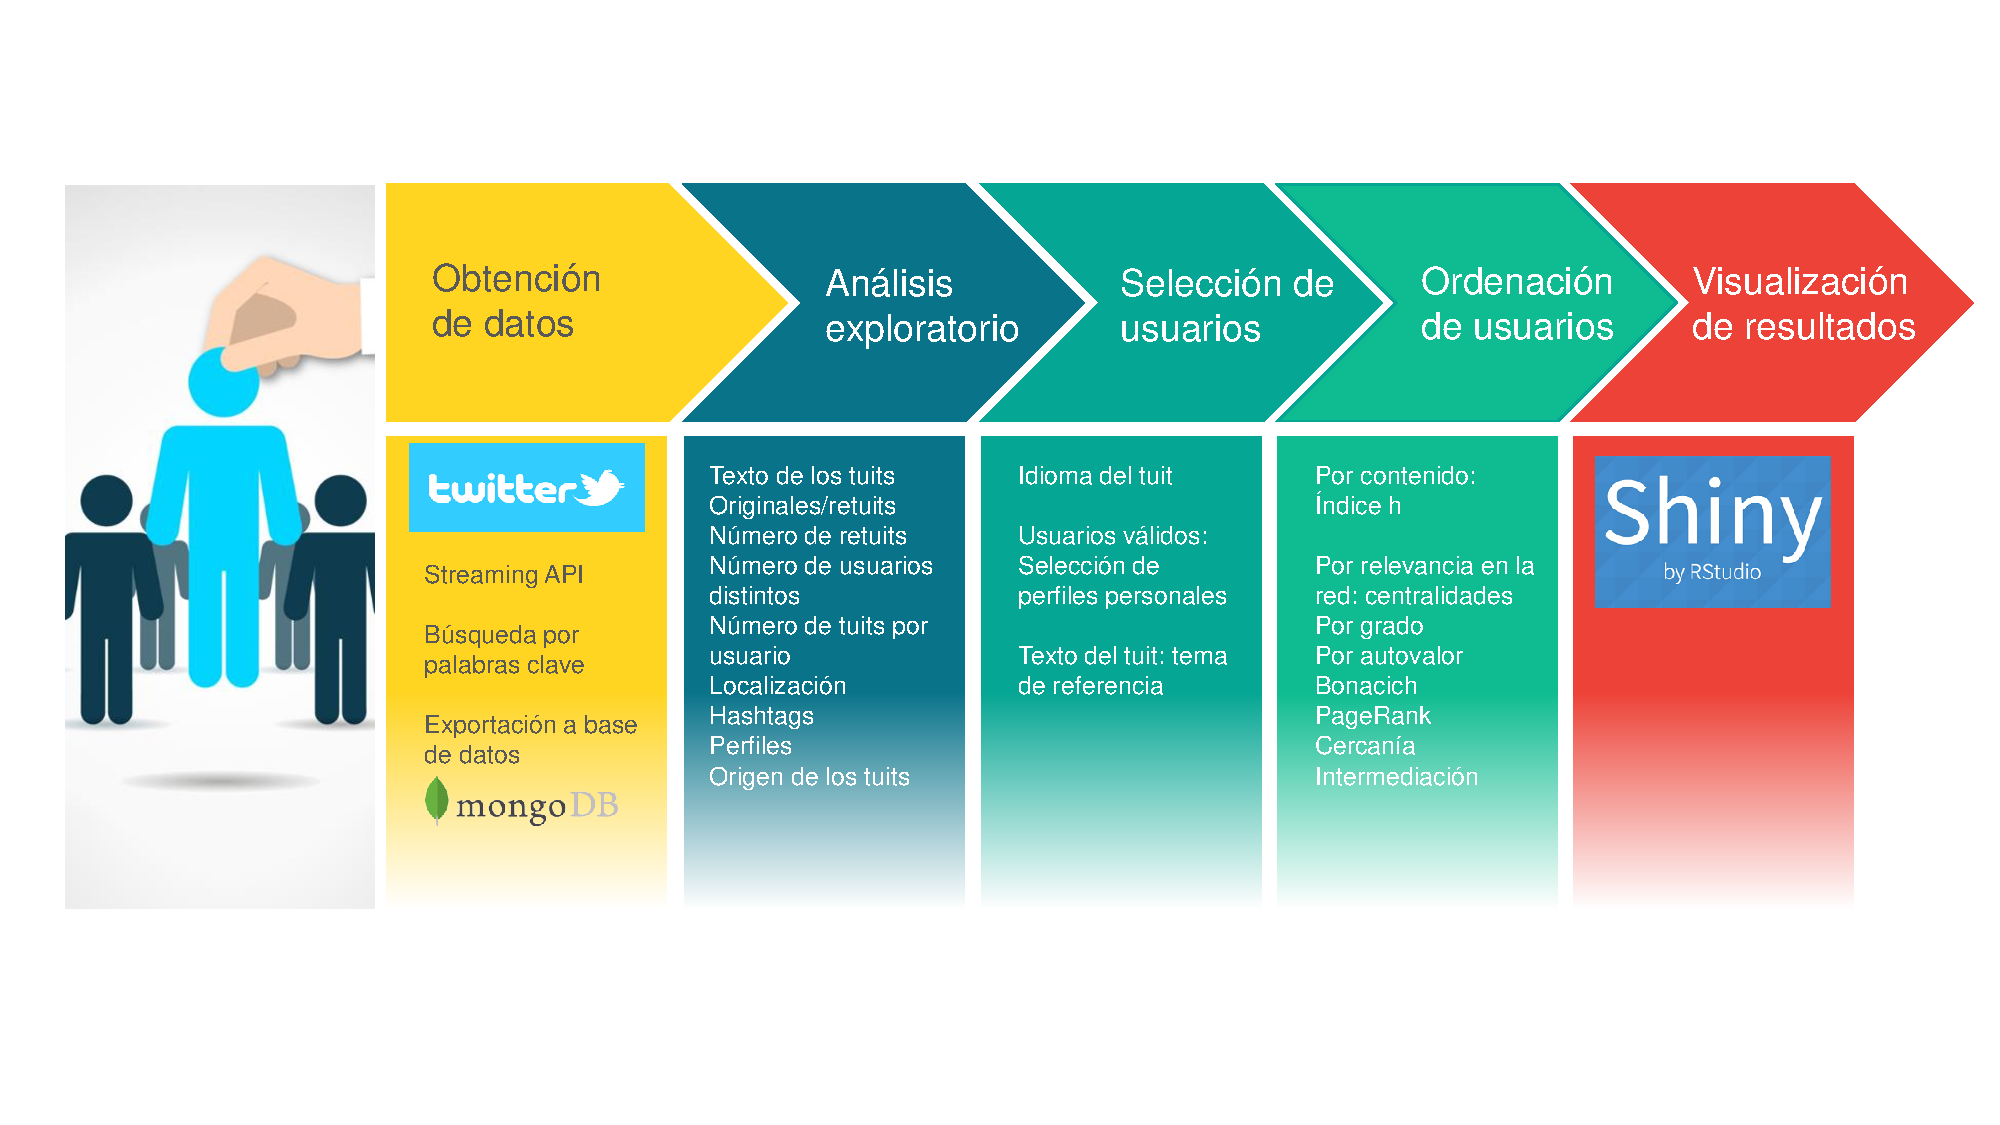
\includegraphics[width=\textwidth]{workflow.pdf}
\caption{Flujo de trabajo esquemático.}
\label{fig:flujo_de_trabajo}
\end{sidewaysfigure}
\chapter*{Executive summary}
\addcontentsline{toc}{chapter}{Executive summary}

\chapter{Planteamiento del proyecto}

En este cap\'\i tulo vamos a describir el contexto en el que vamos a desarrollar el contenido del 
proyecto y las ideas involucradas en su desarrollo.

\section{Descripci\'on}
Cuando un departamento de Recursos Humanos o una empresa de reclutamiento se enfrenta a una petici\'on para
cubrir un puesto vacante o de nueva creaci\'on, el proceso suele llevarse a cabo en diversas fases, que 
podr\'\i amos describir del siguiente modo \cite{proceso_seleccion1}:
\begin{enumerate}
\item {\bf Preselección}: etapa inicial en la que se detectan candidatos adecuados para el perfil buscado, bien recurriendo a 
anuncios en portales especializados, bien con b\'usquedas personalizadas de perfiles. En esta etapa se elabora una lista 
de candidatos que pasar\'an a las siguientes fases del proceso, descartando aquellos cuyas competencias no sean las adecuadas
para el puesto. 
\item {\bf Entrevista inicial}: en esta etapa los candidatos seleccionados en la etapa anterior son contactados para  
conseguir ampliar la informaci\'on de la que se dispone sobre ellos  (por ejemplo sobre las aptitudes
particulares y experiencias previas consignadas en el CV), y verificar el inter\'es y compromiso del candidato
con respecto a la oferta.
\item {\bf Informe}: tras la entrevista inicial, se seleccionan los mejores candidatos para el puesto, y se realiza un informe
donde se consignan los datos originales (el CV, por ejemplo) y los datos a\~nadidos en el curso de la entrevista inicial.
\item {\bf Presentaci\'on de candidatos}: el empleador recibe el informe elaborado en el punto anterior, y selecciona aquellos
que mejor se ajusten a sus necesidades, muy habitualmente realizando nuevas entrevistas con ellos.
\item {\bf Decisi\'on}: es el momento en que se elige el candidato al que se se le va a ofrecer el puesto, etapa en la 
que puede complementarse la informaci\'on recogida hasta el momento con re\-fe\-ren\-cias recabadas de anteriores empleadores.
\item {\bf Oferta}: etapa en la que la empresa presenta al candidato la oferta en firme, habitualmente por escrito, consignando 
la voluntad de la empresa de incorporar al candidato y los detalles econ\'omicos. 
\item {\bf Seguimiento}:  para comprobar que una vez incorporado a la empresa, tanto empleado como empleador est\'an conformes con
el resultado del proceso.
\end{enumerate}

Tradicionalmente, el comienzo de este proceso, la detecci\'on de candidatos, se realizaba en numerosas ocasiones 
a trav\'es de anuncios en prensa,
bases de datos de candidatos construidas a lo largo del tiempo, y la explotaci\'on de la red de contactos personales del entorno 
del empleador. Hoy por hoy, estos m\'etodos tradicionales han sido complementados, y algunos dir\'\i an que pr\'acticamente
suplantados, por m\'etodos que explotan la informaci\'on contenida en la web. 

Los t\'ecnicos de selecci\'on se enfrentan a un mundo muy diverso donde tanto la difusi\'on de los 
posibles puestos como la informaci\'on sobre los candidatos para los mismos est\'a diseminada en numerosos
formatos, teniendo un papel preponderante diversas plataformas o portales web (InfoJobs, Monster, etc.)
y redes sociales en general (LinkedIn, Twitter, Facebook, Instagram, etc.). Desde el punto de vista del t\'ecnico de selecci\'on, las
primeras contienen mucha informaci\'on sobre las aptitudes de los posibles candidatos, sus conocimientos, formaci\'on y 
experiencia, ya que son portales donde los propios usuarios consignan sus curricula vitae, y tambi\'en sobre su situaci\'on laboral
actual y expectativas. En el segundo grupo de fuentes, las redes sociales, hay algunas que tienen el car\'acter espec\'\i fico 
de las primeras (LinkedIn es el ejemplo m\'as claro), y hay otras en las que se consigna informaci\'on diversa, llam\'emoslas de 
prop\'osito general, tal vez en mayor medida personal que profesional.

El objetivo de nuestro proyecto es complementar el 
trabajo habitual de un departamento de Recursos Humanos o de un seleccionador de personal en
los portales y redes sociales dedicados al mundo laboral, con otra informaci\'on laboral extra\'\i da 
de fuentes menos est\'andar, como son las redes sociales de prop\'osito general. 
Estas redes son a menudo aprovechadas por los usuarios para difundir mensajes relacionados con su actividad
laboral, y una descripción de su actividad en las redes es relevante desde el punto de vista 
de un reclutador, en la medida que da informaci\'on del compromiso de la persona con su actividad, su valoración por
parte de otros usuarios, su proactividad, etc.

En este trabajo hemos elegido la red social Twitter por diversos motivos: es una red muy dinámica, fácil de usar, rápida y divertida,
que involucra cientos de millones de usuarios activos en todo el mundo: 328 millones según la web de la red. El crecimiento del número 
de usuarios fue casi exponencial entre 2010 y 2014, si bien últimamente la velocidad a la que adquiere nuevos usuarios ha perido intensidad.
Es también una red que, desde sus orígenes, ha puesto a disposición de los interesados los mecanismos necesarios para acceder a 
la información que atesora, con ciertas limitaciones, pero de forma relativamente sencilla. 



\myfigure{
\begin{tabular}{cc}
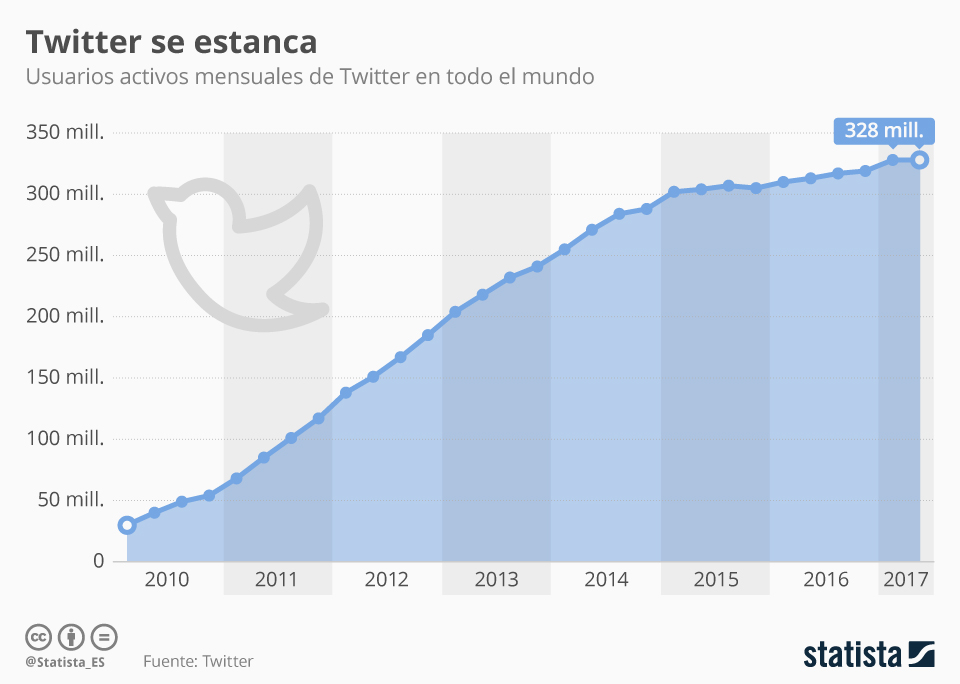
\includegraphics[width=0.4\textwidth]{usuarios_de_twitter}
&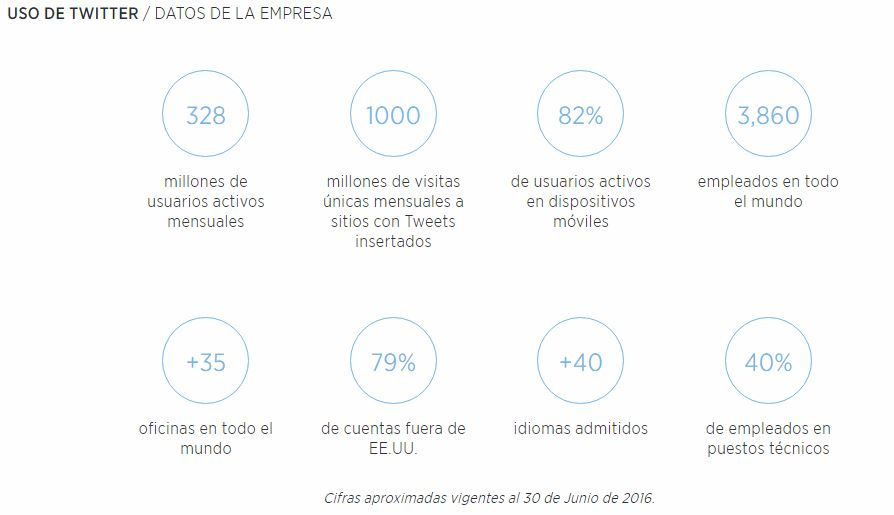
\includegraphics[width=0.4\textwidth]{twitter_uso_y_empresa}
\end{tabular}
\figcaption{Twitter: evolución del número de usuarios (Statista 2017, 
            \url{https://es.statista.com/grafico/10476/el-numero-de-usuarios-de-twitter-se-estanca })
			y datos de la empresa, \url{https://about.twitter.com/es/company }.}
\label{fig:Twitter_uso} }


Esta red da cabida a relaciones diversas, entre usuarios de variada índole, y en particular
muchos de los usuarios  publican información relacionada con su ocupación laboral. Esperamos
detectar en Twitter comunidades de individuos que comparten interés en diferentes 
aspectos de dicho ámbito laboral, con el objetivo de definir e 
implementar un proceso que permita extraer información referente a 
esas comunidades para contribuir a un determinado proceso de selección.

Observemos las dos siguientes ofertas de trabajo aparecidas recientemente (Septiembre 2017) en LinkedIn,
incluyendo los requisitos solicitados a los posibles candidatos:

\myfigure{\begin{tabular}{cc}
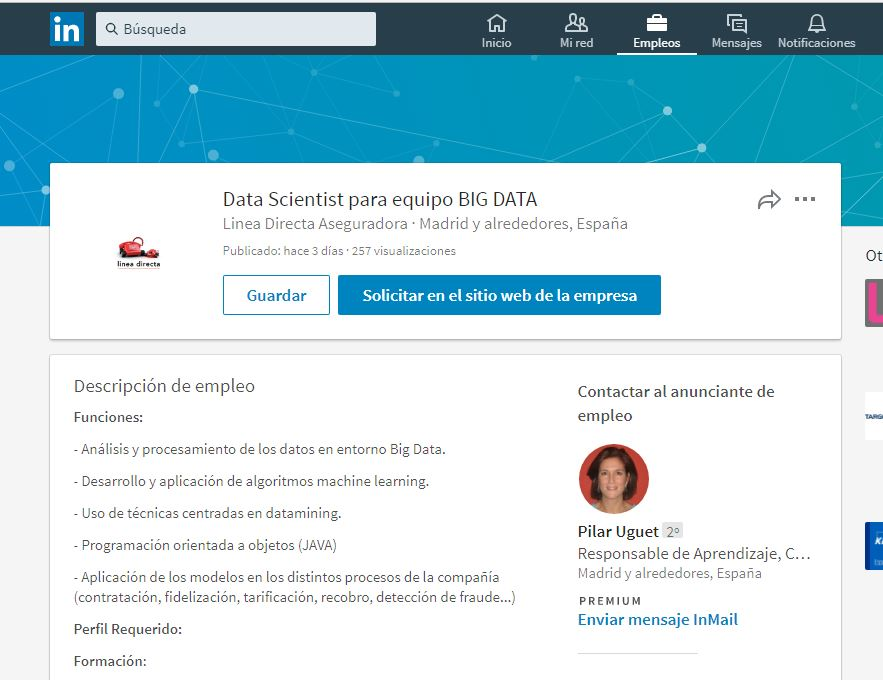
\includegraphics[width=0.4\textwidth]{oferta1_1}
&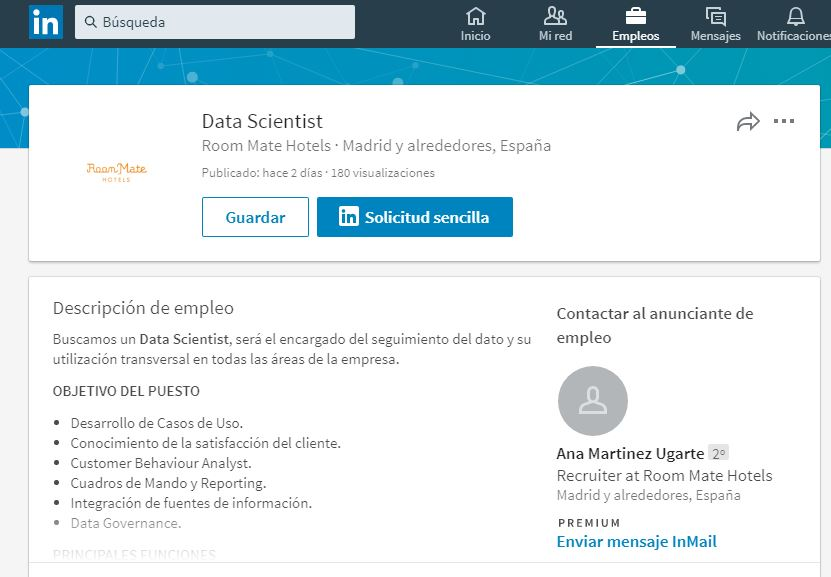
\includegraphics[width=0.4\textwidth]{oferta2_1}
\end{tabular}
\figcaption{Dos ofertas de empleo.}
\label{fig:ofertas_descripcion} }


\myfigure{\begin{tabular}{cc}
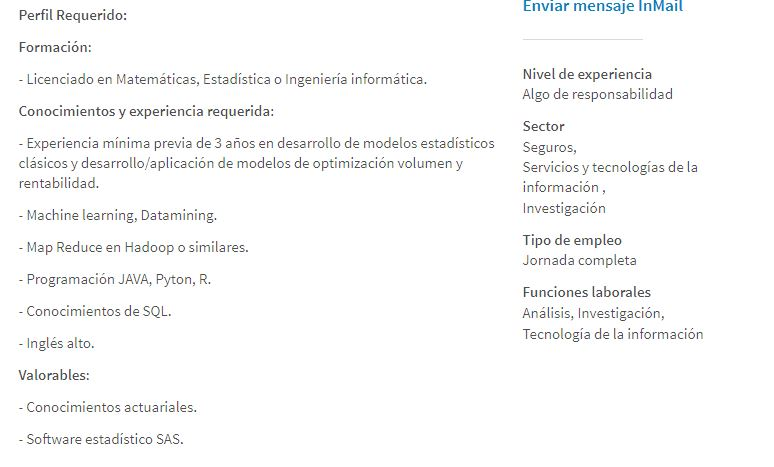
\includegraphics[width=0.4\textwidth]{oferta1_2}
&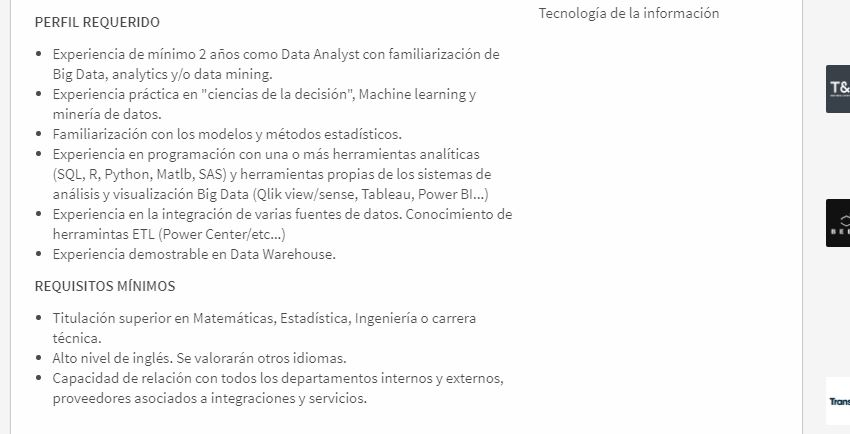
\includegraphics[width=0.4\textwidth]{oferta2_2}
\end{tabular}
\figcaption{Requisitos de las dos ofertas de empleo.}
\label{fig:ofertas_requisitos} }

En ambos casos, entre los requisitos se encuentran conocimientos sobre Python, R,
SQL, machine learning y data mining. Un reclutador probablemente usará esas palabras clave para buscar
los perfiles adecuados para alguno de los dos puestos, y construirá un conjunto de posibles candidatos (el
primer paso en nuestra descripción del proceso de contratación). En esta fase, y gracias a Octopus Data Insights,
nuestro reclutador contará con una ayuda extra. Octopus Data Insights le proporcionará una lista de usuarios
de Twitter que hayan publicado contenido en el que aparezcan esas palabras clave, que complementarán
el resultado que el reclutador haya obtenido por sus propios medios. La información proporcionada
por Octopus Data Insights resultará relevante también más adelante en el proceso,
cuando haya que tomar una decisión entre varios candidatos para determinar cuáles son los más adecuados para el 
puesto: usando la información de Twitter, los usuarios de la lista estarán ordenados según 
diversos criterios de relevancia.

El proceso para producir la información que ayudará al reclutador en el proceso es el siguiente:
\begin{enumerate}
\item Identificar los vocablos que determinan las habilidades que ha de poseer cualquier candidato
para la oferta en cuestión y extraer de Twitter aquellos tuits con contenido relacionado con ellos.
\item Dados esos tuits, construir un conjunto de usuarios, que entendemos como posibles candidatos 
a la oferta.
\item Usar la información publicada por los usuarios para determinar la relevancia del candidato
en función del impacto de sus publicaciones.
\item Estudiar la relación entre los usuarios de este conjunto, y determinar los más relevantes en sentido
relativo (en términos de actividad en la red, cuáles son los más ``retuiteados", cuáles los más seguidos, etc.).
\end{enumerate}



\section{Contexto de negocio}
El área de Recursos Humanos de una compañía, incluso de una de las grandes\footnote{O
una empresa de {\em head hunting}, aunque en esta sección nos referimos solo a departamentos
de RRHH.}, no es el primer área 
en la que suele pensarse cuando hablamos de aplicaciones de las técnicas Big Data en el mundo
empresarial. En general,
parece difícil que los departamentos de RRHH de las compañías,  incluso de las mayores, produzcan
tradicionalmente tanta información propia como para necesitar el software y las herramientas especiales
que las técnicas Big Data proporcionan\footnote{\url{https://hbr.org/2017/06/theres-no-such-thing-as-big-data-in-hr }}:
muchas compañías tienen miles, no millones, de empleados, y la información que recogen con respecto a ellos suele ser anual o cuatrimestral. En algunas ocasiones, el problema puede estar más incluso en
poder acceder a los datos de forma unificada (por el uso de distintos sistemas de almacenamiento),
y en entender y respetar las restricciones legales que aplican a los datos personales de los empleados
a la hora de manejarlos y trasladar los resultados a otros departamentos.

Sin embargo, es notorio el eco que este tipo de técnicas y su aplicación en el área de 
recursos humanos está teniendo recientemente, incluso en prensa generalista:

\begin{center}

\begin{minipage}{0.75\linewidth}
\begin{itemize}

\item[{\bf El País}] Transformación digital y Recursos Humanos: siete reflexiones \newline
\url{ https://retina.elpais.com/retina/2017/12/19/tendencias/1513661663_430453.html }
\item[{\bf ABC}] El Big Data revoluciona los Recursos Humanos \newline
\url{http://www.abc.es/economia/abci-data-revoluciona-recursos-humanos-201609021552_noticia.html }
\item[{\bf Expansión}] Segundo estudio en España sobre transformación digital en RRHH 
\newline \url{ http://www.expansion.com/blogs/lideres-digitales/2017/07/24/2-estudio-en-espana-sobre-transformacion.html }
\item[{\bf ABC}] La revolución tecnológica llega a los recursos humanos pero necesita un cambio cultural
\newline \url{ http://www.abc.es/tecnologia/informatica/soluciones/abci-revolucion-tecnologica-llega-recursos-humanos-pero-necesita-cambio-cultural-201706151516_noticia.html }
\item[{\bf Computerworld}] Meta4 reinventa su propuesta de gestión de recursos humanos\newline 
\url{ http://www.computerworld.es/innovacion/meta4-reinventa-su-propuesta-de-gestion-de-recursos-humanos }
\item[{\bf El Economista}] Por qué Recursos Humanos es un departamento clave en la transformación digital \newline
\url{ http://www.eleconomista.es/firmas/noticias/8523518/07/17/Por-que-Recursos-Humanos-es-un-departamento-clave-en-la-transformacion-digital.html }
\end{itemize}

\end{minipage}
\end{center}


Desde que los primeros departamentos de Recursos Humanos aparecieron (en Estados Unidos
en los primeros años del siglo XX\footnote{\url{http://www.whatishumanresource.com/the-historical-background-of-human-resource-management }}),
se ha estudiado mucho la labor y la función de estos departamentos dentro de las organizaciones
empresariales, y las mejores técnicas y recursos para llevarlos a cabo, y existe abundante bibliografía
al respecto (ver, por ejemplo \url{http://www.whatishumanresource.com/hrm-text-books } para una
primera aproximación). Seguramente, la componente humana del profesional de RRHH no puede ser sustituida
en numerosas circunstancias. Sin embargo, el cambio que las tecnologías digitales
suponen en todos los ámbitos de la actividad humana sin duda impacta en las
actividades de los departamentos de RRHH. Además, el principal uso del Big Data y del análisis
de datos debe ser la ayuda en la toma de decisiones, idealmente en todos los niveles
organizativos. Y es en los departamentos de RRHH donde se toman muchas decisiones sobre el
activo más valorable que compone las organizaciones: las personas. \lq\lq People analytics\rq\rq
es el nombre que recibe la aplicación de las técnicas y tecnologías de Big Data y ciencia de
datos al área de la gestión de personas\footnote{También  \lq\lq workforce analytics\rq\rq, 
\lq\lq talent analytics\rq\rq, \lq\lq human capital analytics\rq\rq, 
\lq\lq talent management analytics\rq\rq, entre otros.}. 

Es por ello que el proceso de transformación digital de las empresas también
debiera incluir a los departamentos de Recursos Humanos, aprovechando los beneficios 
que les podría aportar un enfoque fundamentado en los datos para acometer su tarea.
Puede encontrarse abundante discusión en la red acerca del papel que las tecnologías y
técnicas Big Data pueden jugar en el área de RRHH\footnote{Entre muchos otros:

\noindent\url{https://www.business.com/articles/how-to-utilize-big-data-for-human-resources/ }, 

\noindent\url{https://blog.cake.hr/8-ways-use-hr-analytics-big-data-workplace/ }, 

\noindent\url{http://searchhrsoftware.techtarget.com/feature/Ready-or-not-here-comes-HR-analytics }, 

\noindent\url{https://www.forbes.com/sites/forbeshumanresourcescouncil/2017/02/02/six-powerful-ways-your-hr-team-can-leverage-big-data/\# 282624d65de9 }, 

\noindent\url{http://www.digitalistmag.com/future-of-work/2017/08/31/5-powerful-ways-hr-can-leverage-big-data-05242673 }, 

\noindent\url{https://www.villanovau.com/resources/hr/the-role-of-big-data-in-hr/\# .WkVNst_ibtQ }, 

\noindent\url{https://www.villanovau.com/resources/hr/big-data-changing-hr/\# .Wkdf39_ibtQ }, 

\noindent\url{https://www.cornerstoneondemand.com/glossary/big-data-hr }
} y también recientes estudios que intentan formalizar y dar contexto a dicho papel \cite{libro_rrhh}.
Entre otros, algunos de los aspectos de la labor de los departamentos de RRHH en los que
la aplicación de la tecnología Big Data puede ser de utilidad son los siguientes:
\begin{itemize}
\item \label{item:puntodeproyecto} Procesos de selección: incorporando datos de redes sociales y portales de empleo,
los procesos de selección pueden ser más específicos y eficientes en encontrar candidatos 
adecuados a las posiciones ofertadas. Este punto tiene gran importancia, puesto que
las pérdidas debidas a una mala contratación pueden ser cuantiosas\footnote{\url{https://www.entrepreneur.com/article/244730 }}.
\label{item:puntodeproyecto}

\item Factores de calidad en la contratación: las técnicas Big Data pueden ayudar a los profesionales de
RRHH a determinar qué factores en la trayectoria de un posible candidato son o no importantes a 
la hora de valorar su adecuación a un puesto dado y su rendimiento posterior. A veces, factores que
en principio pueden percibirse como muy importantes (años de experiencia pasada, si esa experiencia fue
en puestos similares o no,\dots) pueden en realidad ser irrelevantes a la luz de los datos disponibles
en la compañía (y cada una, en cada sector y momento, es distinta).

\item Formación y evaluación: no se trata solo de contratar a los mejores candidatos, sino
de que las personas se adapten pronto a sus nuevas labores y al nuevo entorno de trabajo,
y mantener una continua formación que permita al trabajador adaptarse a los cambios en dicho
entorno. Con las técnicas de análisis de datos, puede ser más fácil decidir qué formación es 
la más adecuada para cada profesional, y evaluar los beneficios de dicha formación.

\item Retención de los empleados: evaluando el historial de la compañía,
las técnicas de análisis de datos pueden ayudar a identificar las causas por las que un empleado
deja de formar parte de la misma. A partir de ahí, se pueden identificar aquellos que no 
permanecerán en la compañía, así como aquellos factores que mejor funcionan para retener a los empleados,
y potencialmente optimizar el uso de los recursos destinados a su fidelización. 
Medir la percepción de la sociedad de la compañía como lugar de trabajo a través de las impresiones
reflejadas en redes sociales, por ejemplo, también puede ayudar a los profesionales de RRHH a
identificar áreas de mejora o áreas a potenciar,
a la hora de atraer candidatos para nuevos puestos y retener a los trabajadores.

\item Medida del desempeño: las técnicas de análisis de datos también pueden ayudar a medir
el desempeño de los empleados de forma más precisa, por ejemplo determinando la relación entre 
franjas horarias trabajadas y rendimiento, identificando a los trabajadores más productivos de
forma absolutamente objetiva, o llevando a cabo evaluaciones del desempeño
más frecuentes que anualmente o trimestralmente. Otro aspecto importante en este punto es el uso de dispositivos 
encaminados a monitorizar la actuación de los trabajadores: por ejemplo, plataformas de escucha 
{\em online} para seguir en tiempo real el desempeño en un {\em call center}, o ayudar a los trabajadores
en el trascurso de su quehacer. Este tipo de dispositivos también puede ayudar a los departamentos
de RRHH a cuidar estrechamente la seguridad del trabajador, el cumplimiento de las políticas
de buenas prácticas, etc.

\item Compensación monetaria: el dinero que ganan los empleados con su trabajo es un
factor básico de la satisfacción del empleado. Usando el análisis de datos, los equipos de 
RRHH pueden desarrollar un modelo financiero optimizado. Esto es especialmente importante
en compañías grandes, con empleados en distintas geografías, donde resulta difícil comparar 
los distintos departamentos internacionales. Y es importante en cualquier compañía tener
una guía de cómo realizar una promoción adecuada de los trabajadores optimizando
los costes asociados.

\item Planificación: el análisis de datos puede ayudar a las compañías a identificar tendencias y 
pla\-ni\-ficar acciones. Por ejemplo, se pueden detectar épocas de mayor absentismo por cuestiones de 
salud e implementar políticas para paliarlo (de prevención sanitaria o de contratación de refuerzos), o 
detectar factores que conducen a una mayor incidencia de accidentes que pueden afectar a la producción
y programar acciones para remediarlo.

\end{itemize}

En general, el uso de técnicas de análisis de datos y Big Data, ayudará a cambiar el enfoque
de los departamentos de RRHH a un papel más proactivo, y a ampliar el rango de herramientas en las
que apoyarse al tomar decisiones. En \cite{talent_an} las autoras reflejan varios ejemplos
de compañías donde ya se está aplicando analítica avanzada para solucionar diversos problemas
de los arriba mencionados.

El abanico de aplicaciones enfocadas a la gestión de Recursos humanos es bastante amplio
(en \url{https://www.capterra.com/human-resource-software/ } podemos encontrar una lista con
varias aplicaciones y soluciones enfocadas a este tema), y van desde soluciones propuestas
por proveedores generales de tecnología Big Data y análisis de datos,
como las de Oracle y SAP, a sistemas propuestos por proveedores más especializados, 
como SumTotal Systems, PeopleFluent, Cornerstone, Talent Analytics, CakeHR.
Algunas compañías han desarrollado soluciones propias,
por ejemplo el {\em Project Oxygen} de Google, enfocada a evaluar la actividad de los managers y 
ayudarlos en su desempeño.

Nuestro proyecto se encuadra dentro del primer punto mencionado en la página 
\pageref{item:puntodeproyecto}, y el objetivo es, como ya se ha mencionado,
ayudar en la labor de localizar candidatos a un puesto de trabajo
a través de la extracción y análisis de información de Twitter.

El nuestro es por tanto un proyecto que clasificará perfiles de usuarios de Twitter.
Numerosos  trabajos han explorado la clasificación de usuarios de Twitter
atendiendo a su actividad (ver \cite{tesis_mariluz} y las referencias
incluidas, \cite{user_class5}), para descubrir 
características de usuarios como etnia o género (\cite{user_class1}, \url{https://www.kaggle.com/crowdflower/twitter-user-gender-classification }),
para clasificar la orientación política (\cite{user_class2}) o 
detectar usuarios similares adecuados para seguir (\cite{user_class3}),
detección de bots (\cite{user_class4}), entre otros enfoques.
 

En cuanto a aplicaciones que extraigan información de Twitter y proporcionen 
algún tipo de clasificación de usuarios, podemos encontrar una amplia variedad.
Algunas de las más comentadas en la red son las siguientes:
\begin{itemize}
\item StatusPeople.com: analiza los seguidores de una cuenta de Twitter y los clasifica como buenos, malos o inactivos.
\item Mentionmapp: crea un mapa interactivo que dibuja por menciones, la interacción de una cuenta de Twitter con las últimas 200 publicaciones de la cuenta. Sirve para determinar la calidad de la audiencia en Twitter y poder detectar y diferenciar entre seguidores, fans y superfans.
\item Audiense (antes SocialBro): es una herramienta para identificar audiencias relevantes (de dónde proceden los followers, en qué idioma escriben, si sus cuentas son públicas o privadas, si son cuentas verificadas, identifica seguidores inactivos, etc.). También examina el contenido psicolingüístico de los tuits y permite a las marcas conocer los rasgos de personalidad que están detrás del comportamiento de compra de los usuarios.
\item Twitter Audit: analiza una cuenta tomando como referencia 5.000 seguidores del usuario y le asigna una puntuación según el número de tuits, la fecha del último tuit y la proporción de seguidores/seguidos. Y a continuación, asigna un porcentaje de \lq\lq veracidad\rq\rq de los seguidores de dicha cuenta.
\item Untweeps: averigua qué seguidores de una cuenta no han tuiteado en los últimos 30 días, y facilita dejar de seguirles.
\item Followerwonk: busca usuarios por palabras clave en sus biografías de los usuarios y los muestra por orden de influencia, pudiendo filtrar por localización, número de followers, número de Tweets, etc. 
\item Buzzsumo: esta herramienta sirve para localizar usuarios influyentes en Twitter a partir de palabras clave o para medir el rango de influencia de una persona o marca en concreto. 
\item Klear: también para localizar usuarios influyentes en diversas plataformas, además de Twitter.
\item Trolldor: ofrece una lista negra de cuentas de Twitter clasificadas como falsos usuarios influyentes o trolls.
\item Klout: puntúa el perfil social según su influencia y facilita una lista de las bios más influyentes según la temática. Propone contenidos para mejorar la puntuación de una cuenta.
\item Peerindex: también ayuda a encontrar usuarios influyentes, en diversas redes sociales además de Twitter.
\end{itemize}

Hasta donde conocemos, no hay ninguna aplicación, comercial o no, 
ni trabajo académico, que tenga la misma orientación que el proyecto 
que desarrollamos. Hay, por supuesto, referencias en las que nos apoyaremos
para clasificar el lenguaje de los tuits y descripciones, para determinar qué perfiles
son personas, y para clasificar el texto de los tuits, así como para luego ordenar
por importancia y relevancia los usuarios detectados (de todas estas referencias hablaremos
más concretamente en cada punto particular). Sin embargo, 
la combinación de técnicas que proponemos en este proyecto no la hemos encontrado,
y en particular, no la hemos encontrado enfocada al objetivo planteado: encontrar
posibles candidatos relevantes para una oferta de trabajo a partir de
la actividad relacionada en Twitter.



\section{Objetivos y criterio de éxito}
Como hemos mencionado anteriormente, nuestro objetivo final es proporcionar una lista de usuarios de Twitter que hayan publicado contenido relacionado con una oferta de trabajo, ordenados por relevancia, de forma que un reclutador pudiera usarla para contactar con ellos e incluirlos en su proceso de selección.

Nuestro criterio de éxito es por tanto conseguir dicha clasificación de los usuarios,
y aportar valor con un método propio, particularizable y eficiente, para conseguirlo. 

\section{Hip\'otesis y limitaciones}
La hipótesis fundamental que estamos haciendo al iniciar este proceso, es que la actividad en Twitter
acerca de un determinado tema (por ejemplo, publicar algo relacionado con Python), supone
que el usuario en cuestión tiene conocimientos sobre dicho tema (en nuestro caso, entenderíamos que ese
usuario posee conocimientos de Python). Esto es cuestionable, por supuesto, pero también ponderable
si tenemos en cuenta que la actividad no sea esporádica. Si un usuario publica sobre un tema
en numerosas ocasiones, la hipótesis de que ese tema no le resulta ajeno, va cobrando fuerza.

Entre las limitaciones de las que adolece el proceso definido para llevar a cabo el proyecto, se encuentran las 
siguientes:
\begin{enumerate}
\item En general, no todos los posibles candidatos tienen por qué usar Twitter, y por tanto habrá muchos que 
queden directamente fuera de nuestro proceso.
\item Los tuits utilizados en el proceso están sujetos a una ventana temporal. Habrá muchos candidatos,
usuarios de Twitter, que no aparezcan en nuestros registros, por no presentar actividad durante ese tiempo.
\item Twitter impone limitaciones en la cantidad de información a la que deja acceder, y por ello, también es
posible que los usuarios pierdad visibilidad en este proceso, 
porque el contenido publicado por ellos no se encuentre entre el proporcionado por la red social durante el proceso
de extracción de datos.
\end{enumerate}


Otra limitación del proceso es que la información que obtenemos de la red es a nivel de usuario de Twitter. 
La dirección de correo o el nombre verdadero de la persona en cuestión, o cualquier dato que pudiera identificarla
no está necesariamente disponible en la aplicación, salvo que el usuario lo haya querido hacer público explícitamente. 
Esta información, y la forma en que se utilice, es clave para la usabilidad del resultado del proyecto, en dos aspectos principales:
\begin{enumerate}
\item para que el reclutador pueda hacer uso de la información, la persona ha de estar identificada, lo suficientemente
como para abrir un canal de comunicación entre el reclutador y el posible candidato.
\item Desde el punto de vista de la comercialización del resultado del proyecto, el hecho de identificar usuarios en una red
social y usar esa información con fines lucrativos, ha de ser implementado de forma muy cuidadosa. El impacto de la Ley 
Orgánica de Protección de Datos de Carácter Personal (LOPD) es muy relevante en nuestro proyecto, y merece un apartado especial.
Nos ocupamos de ello en la sección \ref{subsection:LOPD}.
\end{enumerate}
En relación al primer punto, evidentemente proporcionar un usuario de Twitter ya es abrir un canal de
comunicación. Sin embargo, solo la información de las publicaciones del usuario no es suficiente para 
incluirlo en un proceso de selección, incluso antes del primer contacto entre reclutador y candidato,
y el primero probablemente  necesitará más información (por ejemplo un CV) para considerar al segundo. 
Una forma de solventarlo sería cruzar la información de Twitter (el nombre de usuario)
con la contenida en otros portales (como LinkedIn,  Facebook, Academia.edu, ResearchGate, Glassdoor, etc.),
ya que a menudo el usuario de Twitter es parte de los datos consignados en los CV. Esta extensión
del proyecto la hemos dejado deliberadamente fuera del planteamiento de este proyecto, aunque sería 
{\em conditio sine qua non} para una implementación comercializable del proyecto.




\subsection{La Ley Orgánica 15/1999, de 13 de diciembre, de Protección de Datos
de Carácter Personal}
\label{subsection:LOPD}

Conviene aquí destacar que ninguno de los componentes del equipo de Octopus Data Insights 
tiene la formación ni la experiencia adecuadas para emitir un juicio sobre la aplicación
de la LOPD en un contexto de negocio, y que lo que aquí se expone es fruto de una 
investigación {\em ad-hoc}
para nuestro caso. Es posible que alguna de las opiniones o valoraciones emitidas en esta
sección no sean lo suficientemente precisas, o incluso que sean  incorrectas.

La Agencia Española de Protección de Datos, AEDP, define un dato de carácter personal del siguiente modo:

\myfigure{
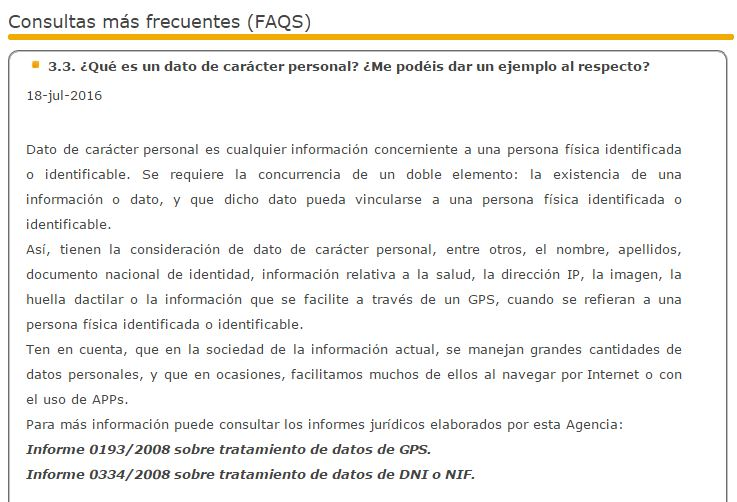
\includegraphics[width=0.6\textwidth]{dato_personal}
\figcaption{AEDP preguntas frecuentes,
           \url{https://sedeagpd.gob.es/sede-electronica-web/vistas/infoSede/detallePreguntaFAQ.jsf;jsessionid=147951A8A98D206E87F2655B9E96E7EB?idPregunta=FAQ%2F00025%
		   }} 
\label{fig:dato_personal} }

El perfil en Twitter de un usuario se puede considerar por tanto un dato de carácter personal, en tanto en cuanto
permitiría localizar e identificar al usuario, tal vez a través de cruces de la información en Twitter con
información adicional (por ejemplo, lo que comentábamos a propósito de encontrar el CV del usuario usando que
frecuentemente, el usuario de Twitter es parte de la información contenida en el mismo, y el CV está disponible en otros 
portales). Sin embargo, en la política de privacidad de Twitter (\url{https://twitter.com/es/privacy })
se establece que
% \begin{center}
% \noindent\begin{minipage}{0.9\linewidth}%{0.9\columnwidth}
% \centering%

\leftskip=1cm
\rightskip=1cm
{\em \lq\lq Al utilizar cualquiera de nuestros Servicios, usted da su consentimiento para la recopilación, 
 la transferencia, la manipulación, el almacenamiento, la revelación y otros usos de su información 
 según lo descrito en esta Política de Privacidad. Esto incluye cualquier información que elija proporcionar que 
 se considere sensible según la legislación vigente.\rq\rq}

\leftskip=0pt\rightskip=0pt
% \end{minipage}
% \end{center}




\noindent Y también, en relación a la información del perfil o publicaciones:
% \begin{center}
% \noindent\begin{minipage}{0.9\linewidth}%{0.9\columnwidth}
% \centering%

\leftskip=1cm
\rightskip=1cm
{\em ''{\bf Información básica de la cuenta}: si opta por crear una cuenta de Twitter, debe promocionar cierta información personal, 
como su nombre, nombre de usuario, contraseña, dirección de correo electrónico o número de teléfono. 
En Twitter, su nombre y nombre de usuario siempre se hacen públicos, incluso en su página de perfil y en los resultados de búsqueda, 
y puede utilizar su nombre real o un seudónimo."}

\leftskip=1cm
\rightskip=1cm
{\em ''{\bf Tuits, gente que sigue, listas, perfil y otra información pública}: Twitter está principalmente diseñado para ayudarle a 
compartir información con el mundo. La mayoría de la información que usted nos facilita a través de Twitter es información 
que nos está pidiendo que hagamos pública. Puede facilitarnos información de perfil para hacerla pública en Twitter, como por 
ejemplo, una breve biografía, su ubicación, su sitio web, fecha de nacimiento, o una fotografía. Además, su información pública 
incluye los mensajes que tuitea; los metadatos facilitados con los tuits, tales como cuándo ha tuiteado y la aplicación cliente 
que utilizó para tuitear; información sobre su cuenta, como el momento de su creación, el idioma, el país y la zona horaria; y las 
listas que crea, las personas a las que sigue, los tuits que retuitea o marca como Me gusta, y las emisiones de Periscope en las que 
hace clic o con las que se relaciona de alguna forma (por ejemplo, haciendo comentarios o clic en el icono de corazón) en Twitter. 
Twitter disemina amplia e instantáneamente su información pública a una amplia gama de usuarios, clientes y servicios, incluyendo 
motores de búsqueda, desarrolladores y editores que integran contenido de Twitter en sus servicios y organizaciones, tales como universidades, 
agencias de salud pública y empresas de investigación de mercado que analizan la información en busque de tendencias y conocimiento."}
% \end{minipage}
% \end{center}

\leftskip=0pt \rightskip=0pt



A tenor de estas afirmaciones, la información que nosotros vamos a manejar en la implementación de este proyecto
(nombre de usuario, información del perfil, tuits publicados)
es una información de carácter público. 

En su enunciado, la LOPD establece que
(texto extraído del informe jurídico  2013-0184 de la AEPD
\url{http://www.agpd.es/portalwebAGPD/canaldocumentacion/informes_juridicos/otras_cuestiones/common/pdfs/2013-0184_Red-social-y-creaci-oo-n-de-perfiles-de-empleados..pdf%
})
% \begin{center}
% \noindent\begin{minipage}{0.9\linewidth}%{0.9\columnwidth}
% \centering%

\leftskip=1cm
\rightskip=1cm
{\em Establece a este
respecto la Ley Orgánica 15/1999 en su artículo 2 que ''El régimen de
protección de los datos de carácter personal que se establece en la
presente Ley Orgánica no será de aplicación: a) A los ficheros
mantenidos por personas físicas en el ejercicio de actividades
exclusivamente personales o domésticas."
}

\leftskip=0pt 
\rightskip=0pt
% \end{minipage}
% \end{center}

\noindent Y define las actividades personales a continuación:

% \begin{center}
% \noindent\begin{minipage}{0.9\linewidth}%{0.9\columnwidth}
% \centering%
\leftskip=1cm
\rightskip=1cm
{\em En cuanto a la determinación de que se entiende por actividades
personales o domésticas dispone el Reglamento de desarrollo de la LOPD en
su artículo 4 que ''Sólo se considerarán relacionados con actividades
personales o domésticas los tratamientos relativos a las actividades que se
inscriben en el marco de la vida privada o familiar de los particulares."
Esta es también la interpretación del término ''personal" contenida en la
Sentencia de la Audiencia Nacional de 15 de junio de 2006 al señalar que ''(…)
Será personal cuando los datos tratados afecten a la esfera más íntima de la
persona, a sus relaciones familiares y de amistad y que la finalidad del
tratamiento no sea otra que surtir efectos en esos ámbitos.}

\leftskip=1cm
\rightskip=1cm
{\em También dará lugar a la aplicación de la Ley Orgánica 15/1999, por
superar el ámbito de la vida privada o familiar de los particulares la publicación
de datos de terceros en la red cuando no existan limitaciones de acceso a su
perfil, en cuanto que dicha publicación constituye una cesión de datos, definida
en el artículo 3 j) de la LOPD como “Toda revelación de datos realizada a una
persona distinta del interesado”, ya que en estos supuestos, como señalaba la
sentencia la Sentencia de 6 de noviembre de 2003 (caso Bodil Lindqvist) del
Tribunal de Justicia de las Comunidades Europeas, no se inscribe en el marco
de la vida privada o familiar de los particulares “un tratamiento de datos
personales consistente en la difusión de dichos datos por Internet de modo que
resulten accesibles a un grupo indeterminado de personas.”}

\leftskip=0pt
\rightskip=0pt
% \end{minipage}
% \end{center}




Refiriéndose incluso a datos de carácter público que aparecen en los datos,
la interpretación de la LOPD respecto al uso de los mismos por terceros, especialmente
en el caso en el que la finalidad de dicho uso sea comercial, es que el único medio
para legitimar el uso es el consentimiento explícito de la persona cuyos datos van 
a utilizarse. Este consentimiento ha de cumplir unas determinadas condiciones
(de nuevo extraemos del informe jurídico  2013-0184 de la AEPD)
% \begin{center}
% \noindent\begin{minipage}{0.9\linewidth}%{0.9\columnwidth}
% \centering%

\leftskip=1cm
\rightskip=1cm
{\em 
El tratamiento de datos de carácter personal debe encontrarse fundado
en alguna de las causas legitimadoras previstas en el artículo 6 de la Ley
Orgánica 15/1999, disponiendo a este respecto su número primero que ''El
tratamiento de los datos de carácter personal requerirá el consentimiento
inequívoco del afectado, salvo que la ley disponga otra cosa."}

\leftskip=1cm
\rightskip=1cm
(\dots)

\leftskip=1cm
\rightskip=1cm
{\em Dicho consentimiento debe reunir las características señaladas en el
artículo 3.h de la misma Ley que lo define como ''manifestación de
voluntad, libre, inequívoca, específica e informada, mediante la que el
interesado consienta el tratamiento de datos personales que le
conciernen".}

\leftskip=1cm
\rightskip=1cm
{\em Esta Agencia ha venido describiendo en sus informes dichas
características de manera que se entiende por consentimiento libre aquel que
ha sido obtenido sin la intervención de vicio alguno del consentimiento en los
términos regulados por el Código Civil.
}

\leftskip=0pt
\rightskip=0pt
% \end{minipage}
% \end{center}


\myfigure{

\includegraphics[width=0.6\textwidth]{LOPD1}
\figcaption{Ayuda Ley de Protección de Datos, 
           \url{https://ayudaleyprotecciondatos.es/2010/09/16/redes-sociales-empresas-y-proteccion-de-datos/ }}
\label{fig:LOPD1} }


Como consecuencia de toda esta información, entendemos lo siguiente:
\begin{itemize}
\item que los datos del perfil de los usuarios de Twitter, así como sus publicaciones en dicha red,
tienen carácter público.
\item Que el carácter público de dichos datos no es óbice para poder manipularlos y distribuirlos
a terceros, en ninguna actividad que no se circunscriba al ámbito personal o familiar.
\item La elaboración de un proyecto de fin de máster no está claro
que pueda entenderse como una actividad del ámbito personal o familiar, con lo cual no estaría en disposición de difundir esa información a terceros, salvo en las condiciones previstas en la LOPD,
a pesar de no perseguir más fines que los didácticos.
\item Cualquier versión comercializable de este proyecto debería contar con los mecanismos
adecuados para obtener el consentimiento explícito de los usuarios para el uso de sus perfiles, 
y posible inclusión en un proceso de selección de personal. Esta fase quedará fuera del plan de elaboración
del proyecto.
\end{itemize}
{\bf\color{oblue}
\label{note:why_only_user_id}
Para eliminar el riesgo relativo a protección de datos en la elaboración del proyecto, 
pero sin alterar su esencia, proponemos publicar los resultados enmascarando los nombres 
de usuario de aquellos que aparezcan en nuestra base de datos. A pesar de no ser una solución
perfecta (hay aplicaciones y páginas web que permiten obtener obtener el identificador de usuario
de Twitter o simplemente id\footnote{Con \lq\lq id\rq\rq nos referiremos al identificador único 
que asigna Twitter a cada usuario, que está asociado a la cuenta del usuario, \url{https://developer.twitter.com/en/docs/tweets/data-dictionary/overview/user-object },
y no puede ser modificado por él salvo creando una cuenta distinta.}
a partir del nombre de usuario, y viceversa), hemos decidido que, salvo 
a efectos exploratotios de los datos, usaremos siempre el id de Twitter de
cada usuario para mostrar los resultados. }

\section{Esquema de desarrollo del proyecto}
En las siguientes secciones de la memoria iremos estudiando y describiendo las distintas
fases que componen el proyecto, que podemos dividir en tres grandes subgrupos:
\begin{enumerate}
\item Comenzaremos por hacer un análisis descriptivo de la base de datos recogida a partir del API de Twitter, en relación con el problema que nos ocupa. Estudiaremos la proporción de tuits originales
frente a retuiteados, número de tuits descargados por día, número de retuits, relación entre el 
número de tuits descargados y el número de usuarios distintos, el número de tuits por usuario, y
los hastags presentes en los mensajes. Esta tarea la llevaremos a cabo en el capítulo \ref{chap:tratamiento_inicial_de_los_datos}.

\item A continuación, comienza la fase de proceso de la información. Nuestro objetivo es 
constuir una lista de usuarios que podamos recomendar a un profesional de Recursos Humanos como
posibles candidatos para una oferta. El primer paso, realizado en el capítulo \ref{chap:extraccion_de_usuarios}, es entonces seleccionar, a partir de la información descargada de Twitter, los usuarios de interés. 

\item La fase siguiente será, con esa lista de usuarios extraídos en la fase anterior, ordenarlos
en función de su comportamiento en Twitter (difusión e interacción con otros usuarios). 
La metodología empleada en este apartado, así como una descripción de los resultados, 
se abordan en el capítulo \ref{chap:ordenacion_de_usuarios}.

\item Por último, pero no menos importante, desarrollaremos la fase de visualización de los
datos, para aportar usabilidad a los resultados del proyecto, fase descrita en el
capítulo \ref{chap:visualizacion}
\end{enumerate}

Este esquema corresponde con el esquema de la llamada general a las distintas funciones que se
ejecutan en el proyecto (en el fichero {\bf Python/master.py} del repositorio, ver la sección
\ref{sect:repositorio}):

\myfigure{
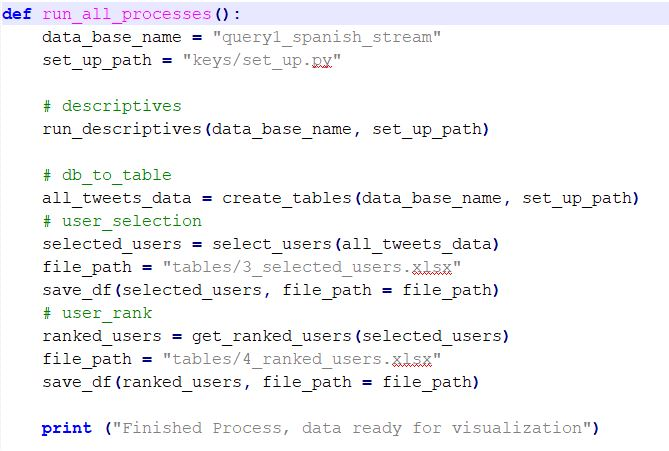
\includegraphics[width=0.7\textwidth]{master_sucessive_calls}
\figcaption{Llamadas a las funciones de procesado de la información}
\label{fig:master_sucessive_calls} }
\chapter{Planificación del proyecto}
\section{Equipo}
El equipo de Octopus Data Insights está formado por cuatro personas, con perfiles multidisciplinares y complementarios:
\begin{itemize}
\item Fabio Inui: 
\item Teresa Martínez: matemática, con diez años de experiencia en investigación y docencia a nivel universitario,
ocho en construcción de modelos de valoración de derivados en empresa financiera de primer nivel, y cuatro de
gestión de fondos en una de las principales gestoras españolas.
\item Javier Quintana: 
\item Silvia Santos: 
\end{itemize}
\section{Desarrollo temporal}



\chapter{Infraestructura}
En esta sección describiremos la infraestructura que hemos construido para el desarrollo del proyecto.
\section{Repositorio GIT}
\label{sect:repositorio}
El código del proyecto, así como las presentaciones y memoria de este proyecto, está almacenado en el 
repositorio \url{https://github.com/MaiteMartinez/MBITProject_Data4all}

\myfigure{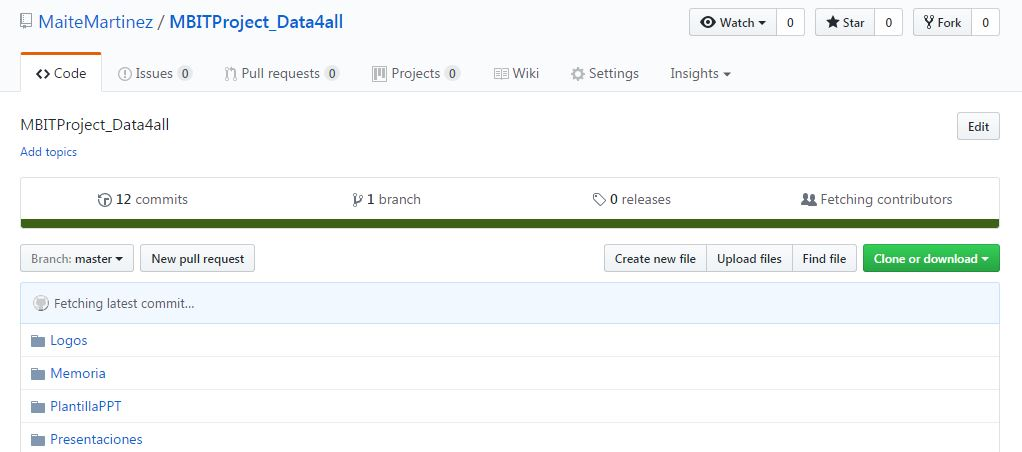
\includegraphics[width=0.6\textwidth]{repositorio_git1}%
\figcaption{Repositorio del código del proyecto.}
\label{fig:repositorio_git1} }

\section{Infraestructura para la obtención de datos}

Como muchas redes sociales, Twitter ofrece acceso a la información que generan sus usuarios a través de un
API ({\em Application Programming Interface})\cite{twitter_dev_web}. El API de Twitter ofrece diversas opciones: 
Webhook APIs, ADS API, REST APIs y Streaming APIs. La primera está enfocada a generar  
notificaciones instantáneas a partir de detección de eventos y la segunda a la integración de aplicaciones con la 
plataforma de publicidad de Twitter. Para nuestro proyecto, solo son relevantes por tanto las dos segundas:
\begin{itemize}
\item El API Rest ({\em Representational State Transfer}) permite realizar consultas puntuales con los parámetros de búsqueda indicados,
a través de una componente denominada Search API. El Search API funciona de manera similar, aunque no 
exactamente igual, a la búsqueda en la página web de Twitter. El Search API 
realiza la búsqueda entre una muestra de tuits publicados en los últimos siete días, y
las búsquedas están limitadas a 180 peticiones cada ventana temporal de 15 minutos. 

\myfigure{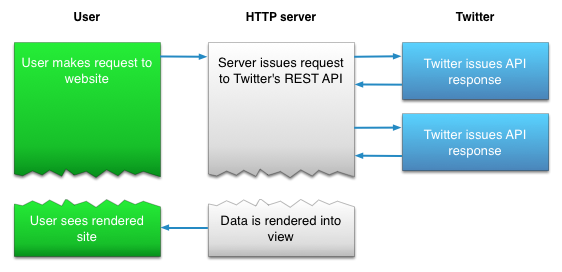
\includegraphics[width=0.6\textwidth]{api_rest_como_funciona}%
\figcaption{Funcionamiento del API Rest. \url{ https://dev.twitter.com/streaming/overview}}
\label{fig:api_rest_como_funciona} }

La búsqueda realizada por este API está centrada en la relevancia y no en la completitud, lo que 
quiere decir que algunos tuits y usuarios podrían quedarse fuera.

\item El API Streaming permite un acceso con baja latencia al flujo global de tuits de la aplicación,
y requiere una conexión HTTP continua. Entre los tipos de flujos disponibles, en la web de Twitter
para desarrolladores, se recomienda usar los flujos públicos para realizar minería de datos (en dichos flujos
aparecen muestras de los datos públicos de Twitter).

\myfigure{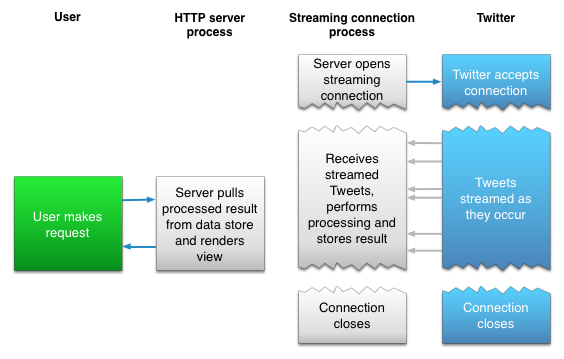
\includegraphics[width=0.6\textwidth]{api_streaming_como_funciona}%
\figcaption{Funcionamiento del API Streaming. \url{ https://dev.twitter.com/streaming/overview}}
\label{fig:api_streaming_como_funciona} }

\end{itemize}

El acceso a ambas versiones de API está gobernado por la autentificación mediante el protocolo OAuth
({\em Open Authorization}), lo que implica que para cada aplicación deben obtenerse los tokens necesarios 
de la sección de desarrolladores de Twitter, estableciéndose un número máximo de 7 por usuario.
También para ambas versiones del API existen restricciones de acceso. Estas restricciones solo
afectan a las versiones gratuitas de los APIs. Hay una versión de pago de este acceso  (Twitter Firehose)
que garantiza como respuesta el 100\% de los tuits que cumplan los criterios de la búsqueda.
Para el desarrollo de este proyecto nos hemos servido del API gratuito, por limitación de costes. 

Entre los API REST y Streaming, hemos decidido utilizar el API Streaming, mediante un script
en Python usando Tweepy. Este método tiene diversas ventajas y desventajas que pasamos
a revisar:
\begin{enumerate}
\item El API Streaming proporciona tuits en tiempo real, y funciona como una especie de \lq\lq grabadora\rq\rq,
con la que se van registrando todos los tuits a medida que se van produciendo.
\item Como es un proceso que se mantiene a la escucha y va reflejando entradas según
se producen, la infraestructura necesaria para que funcione es algo  más complicada que para
el API Search. Se necesita, por ejemplo, una conexión contínua a Internet, ya que el tiempo que
el proceso no esté corriendo, no estaremos recogiendo tuits.
\item El límite de bajada de los tuits en el API Stream es de 50 tuits por segundo.
En nuestro caso, el número de tuits que se producen no pasan de unas decenas por minuto, con
lo cual nos aseguramos un barrido bastante exhaustivo de la actividad relevante.
\item Además, al ir bajando tuits consecutivamente, minimizamos el problema de tener tuits repetidos.
\item Como desventaja, no podemos acceder a tuits antiguos, y solo tendremos aquellos que 
se produzcan en el tiempo que esté el proceso de \lq\lq escucha\rq\rq levantado.
\end{enumerate}

Con respecto al segundo punto, hemos bajado los tuits mediante un script de Python, 
que usa la librería Tweepy, y 
en el que a medida que van llegando los tuits a un proceso de escucha, los vamos 
almacenando en una base de datos MongoDB. 

\myfigure{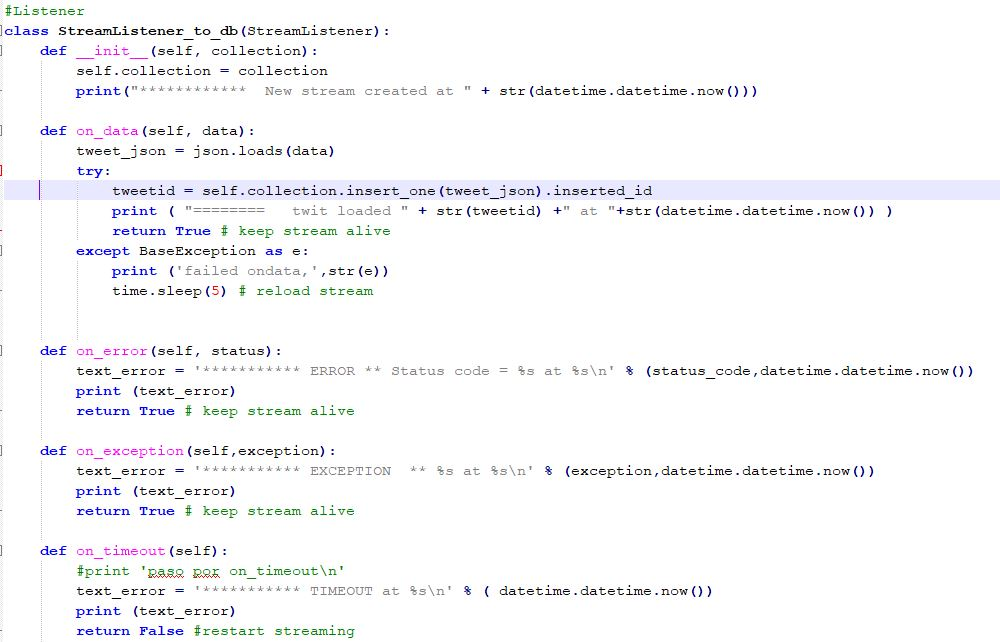
\includegraphics[width=0.6\textwidth]{streamlistener1}%
\figcaption{Función de escucha de tuits.}
\label{fig:streamlistener1} }

Para mantener vivo el proceso de escucha y que no caiga frente a errores o timeouts,
incluimos en el script un control de incidencias:

\myfigure{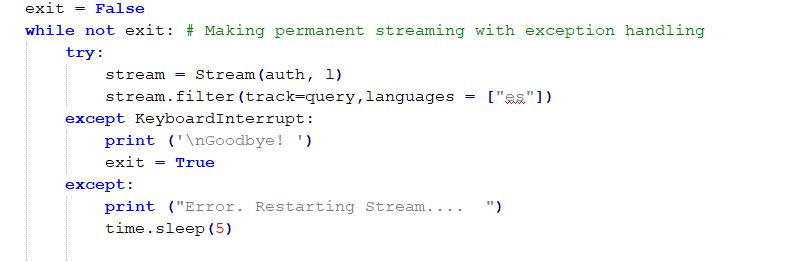
\includegraphics[width=0.6\textwidth]{streamlistener2}%
\figcaption{Gestión de incidencias en el proceso de escucha.}
\label{fig:streamlistener2} }

Y para refrescar el proceso, y que la conexión con Twitter funcione correctamente
de forma continua, se programaron relanzamientos diarios del script en el programador 
de tareas de Windows.
 

Para el desarrollo de la mayor parte de la lógica del proyecto hemos elegido Python 3.6 (a través de la
instalación de Anaconda). Esta elección tiene diversas ventajas, en las varias fases del proyecto, ya
que este lenguaje facilita las siguientes tareas:
\begin{itemize}
\item Comunicación con el API Streaming de Twitter a través del paquete Tweepy.
\item Sencilla interacción con el formato JSON, que es en el que los tuits son descargados desde el API, gracias al paquete json.
\item  Comunicación con la base de datos documental MongoDB, a través del paquete pymongo.
\item Incorporación nativa del encoding UTF-8 (\lq\lq Unicode Transformation Format\rq\rq con números de 8 bits), 
lo que nos ahorra muchos quebraderos de cabeza al tratar con caracteres especiales del español (tildes, ñ, etc.)
y la presencia de emojis en los textos de los tuits.\footnote{\url{https://docs.python.org/3/howto/unicode.html. }}
\end{itemize}

Para la primera toma de contacto con los datos descargados del API de Twitter, nos hemos decantado por 
almacenarlos según íbamos recogiéndolos en una base de datos MongoDB. Las razones son varias:
\begin{itemize}
\item MongoDB trata de forma natural documentos en formato JSON.
\item También maneja sin problemas documentos con encoding UTF-8\footnote{
\url{https://docs.mongodb.com/v3.4/reference/bson-types/ }}, lo que nos ayuda a no tener problemas de encoding al
almacenar los tuits.
\item Se integra muy bien en programas en Python gracias al paquete pymongo.
\item No necesita una definición de la estructura del documento, lo que es muy conveniente
para tratar tuits, donde el número de campos que obtenemos del API y el contenido de esos campos no siempre
sigue el mismo formato. Este punto es en particular relevante si el API de Twitter cambiase, o se introdujeran nuevos 
campos. Por ejemplo: a partir del 26 de Septiembre de 2017,  Twitter cambió el límite de 140 caracteres
a un límite de 280 caracteres a algunos usuarios, y eso provocó que aparecieran nuevos campos en el cuerpo de cada
tuit\footnote{\url{https://developer.twitter.com/en/docs/tweets/tweet-updates }}.
\item Es una base de datos bastante rápida, y escalable.
\end{itemize}

\section{Desarrollo en la nube}
\chapter{Tratamiento inicial de los datos: análisis descriptivo}
\label{chap:tratamiento_inicial_de_los_datos}

\section{Descripci\'on de los datos}


\begin{wrapfigure}[17]{R}{0.5\textwidth}

\includegraphics[width=0.45\textwidth]{tuit_ejemplo}
\caption{Ejemplo de tuit.}\label{fig:tuit_ejemplo}
\end{wrapfigure} 


En pantalla, un tuit relevante para nuestro proyecto podría ser el 
mostrado en la figura ad\-ya\-cente. Sin embargo, cuando descargamos el mismo tuit a través del API Search de Twitter, 
obtenemos mucha más información, en formato JSON. 

El formato JSON ({\em Javascript Object Notation})\footnote{\url{http://www.json.org/json-es.html}} 
es un formato ligero de intercambio de datos, fácilmente interpretable (por humanos y por
máquinas). Es un formato ampliamente utilizado, siendo numerosos los
lenguajes que son capaces de usar este formato (lenguajes de la familia C,Javascript, PHP, Python, etc.). 
En JSON se pueden representar dos tipos
de estructuras: un conjunto de pares (clave,valor) con la sintaxis \{clave1:valor1, clave2:valor2,\dots\}, también
denominado {\em objeto}, y un conjunto ordenado de valores con la sintaxis [valor1, valor 2,\dots] (que se denomina {\em arreglo}). 
Un valor puede ser una cadena de caracteres con comillas dobles, un número, un valor booleano o nulo, 
un objeto o un arreglo. Esta flexibilidad permite representar datos de gran complejidad.

Como veremos en el siguiente ejemplo de un tuit en formato JSON descargado a través del API Search de Twitter,
puede resultar de ayuda pensar en un JSON como en un diccionario \{clave:valor\}, donde las claves
son cadenas de texto, y el valor es algo flexible que acomoda desde una cadena de texto a un vector de objetos 
o un nuevo diccionario. En particular, la información del tuit que considerábamos más arriba 
luce de la siguiente manera:

\bigskip


\{'\_id': ObjectId('59e0cbb03842ed08188233d7'),

\quad'contributors': None,

\quad'coordinates': None,

\quad'created\_at': 'Wed Oct 11 08:13:41 +0000 2017',

\quad'entities': \{'hashtags': [\{'indices': [90, 106],'text': 'MachineLearning'\},

				  \hspace{4cm}\{'indices': [107, 114],'text': 'Python'\}],

	\hspace{2cm} 'symbols': [],

	\hspace{2cm}'urls': [\{'display\_url': 'twitter.com/i/web/status/9…',

				\hspace{3cm}'expanded\_url': 'https://twitter.com/i/web/status/918026805080182785',

				\hspace{3cm}'indices': [116, 139],

				\hspace{3cm}'url': 'https://t.co/1WuwNRzn8z'\}],

	\hspace{2cm}'user\_mentions': []\},

\quad'favorite\_count': 1,

\quad'favorited': False,

\quad'geo': None,

\quad'id': 918026805080182785,

\quad'id\_str': '918026805080182785',

\quad'in\_reply\_to\_screen\_name': None,

\quad'in\_reply\_to\_status\_id': None,

\quad'in\_reply\_to\_status\_id\_str': None,

\quad'in\_reply\_to\_user\_id': None,

\quad'in\_reply\_to\_user\_id\_str': None,

\quad'is\_quote\_status': False,

\quad'lang': 'es',

\quad'metadata': \{'iso\_language\_code': 'es',

	 \hspace{2.3cm}'result\_type': 'recent'\},

\quad'place': None,

\quad'possibly\_sensitive': False,

\quad'retweet\_count': 0,

\quad'retweeted': False,

\quad'source': '\verb|<a href="http://twitter.com"  rel="nofollow">Twitter Web Client</a>|',

\quad'text': 'Vamos preparando el siguiente libro a estudiar que al final la movida 

\hspace{1.7cm}me está gustando... \#MachineLearning \#Python… https://t.co/1WuwNRzn8z',

\quad'truncated': True,

\quad'user': \{'contributors\_enabled': False,

\hspace{1.7cm}'created\_at': 'Sat Dec 12 09:13:46 +0000 2009',

\hspace{1.7cm}'default\_profile': False,

\hspace{1.7cm}'default\_profile\_image': False,

\hspace{1.7cm}'description': 'Me gustan las camisetas y las  zapatillas // Desarrollo y '

\hspace{3cm}'Diseño para sistemas Apple //  Creador de @GetPomodoroApp ·  '

\hspace{3cm}'@GetAtentoApp · @MADatBUS ·  @GetMeteo y...',

\hspace{1.7cm}'entities': \{'description': \{'urls': []\},

\hspace{3.5cm}'url': \{'urls': [\{'display\_url': 'desappstre.com',

\hspace{4.5cm}'expanded\_url': 'http://desappstre.com',

\hspace{4.5cm}'indices': [0,23],

\hspace{4.5cm}'url': 'https://t.co/oYY42NlHrT'\}]\}\},

\hspace{1.7cm}'favourites\_count': 1512,

\hspace{1.7cm}'follow\_request\_sent': False,

\hspace{1.7cm}'followers\_count': 211,

\hspace{1.7cm}'following': False,

\hspace{1.7cm}'friends\_count': 209,

\hspace{1.7cm}'geo\_enabled': True,

\hspace{1.7cm}'has\_extended\_profile': True,

\hspace{1.7cm}'id': 96309647,

\hspace{1.7cm}'id\_str': '96309647',

\hspace{1.7cm}'is\_translation\_enabled': False,

\hspace{1.7cm}'is\_translator': False,

\hspace{1.7cm}'lang': 'es',

\hspace{1.7cm}'listed\_count': 109,

\hspace{1.7cm}'location': 'Madrid — Mundo Real™',

\hspace{1.7cm}'name': 'Adolfo ™',

\hspace{1.7cm}'notifications': False,

\hspace{1.7cm}'profile\_background\_color': '000000',

\hspace{1.7cm}'profile\_background\_image\_url': 'http://abs.twimg.com/images/themes/theme2/bg.gif',

\hspace{1.7cm}'profile\_background\_image\_url\_https': 'https://abs.twimg.com/images/themes/theme2/bg.gif',

\hspace{1.7cm}'profile\_background\_tile': False,

\hspace{1.7cm}'profile\_banner\_url': 'https://pbs.twimg.com/profile\_banners/96309647/1501577205',

\hspace{1.7cm}'profile\_image\_url': 'http://pbs.twimg.com/profile\_images/888396793024794624/O6gHh-lJ\_normal.jpg',

\hspace{1.7cm}'profile\_image\_url\_https': 'https://pbs.twimg.com/profile\_images/888396793024794624/O6gHh-lJ\_normal.jpg',

\hspace{1.7cm}'profile\_link\_color': '1B95E0',

\hspace{1.7cm}'profile\_sidebar\_border\_color': '000000',

\hspace{1.7cm}'profile\_sidebar\_fill\_color': '000000',

\hspace{1.7cm}'profile\_text\_color': '000000',

\hspace{1.7cm}'profile\_use\_background\_image': False,

\hspace{1.7cm}'protected': False,

\hspace{1.7cm}'screen\_name': 'FitoMAD',

\hspace{1.7cm}'statuses\_count': 6893,

\hspace{1.7cm}'time\_zone': 'Madrid',

\hspace{1.7cm}'translator\_type': 'none',

\hspace{1.7cm}'url': 'https://t.co/oYY42NlHrT',

\hspace{1.7cm}'utc\_offset': 7200,

\hspace{1.7cm}'verified': False\}\}

\bigskip

La descripción de cada campo de los que integran el tuit puede encontarse en la página web de Twitter para 
desarrolladores, \url{https://developer.twitter.com/en/docs/tweets/data-dictionary/overview/tweet-object}.

\section{Obtenci\'on de los datos}
Los tuits que componen nuestro corpus de datos los hemos obtenido a través del API Streaming
de Twitter, a través de una búsqueda dirigida en el API Streaming. Esta búsqueda dirigida 
se ha realizado a través de palabras clave, asociadas a la actividad de data science, concretamente:

\begin{center}
\begin{tabular}{ccccc}
\lq\lq machine learning\rq\rq  &\lq\lq machinelearning\rq\rq  &\lq\lq datamining\rq\rq  &\lq\lq data mining\rq\rq 
&\lq\lq Python\rq\rq\\
\lq\lq SQL\rq\rq & \lq\lq hadoop\rq\rq  &\lq\lq bigdata\rq\rq  &\lq\lq big data\rq\rq  &\lq\lq pentaho\rq\rq\\
\lq\lq rstats\rq\rq &\lq\lq SAS\rq\rq &\lq\lq tableau\rq\rq
\end{tabular}
\end{center}

Esta petición se define como un vector en Python, donde la coma significa \lq\lq OR\rq\rq y el espacio
dentro de las comillas significa \lq\lq AND\rq\rq, y se incluyeron dichos términos con y sin almohadilla 
(\#).

También hemos incluido en la búsqueda un filtro por idioma, incluyendo el parámetro 
\lq\lq languages = ["es"]\rq\rq en la llamada al API, con el objetivo de bajar solo tuits
en un idioma. En principio\footnote{\url{https://developer.twitter.com/en/docs/tweets/filter-realtime/guides/basic-stream-parameters }}
esta búsqueda debería devolver tuits que la aplicación Twitter ha detectado como escritos en
idioma español. Sin embargo, también bajamos tuits en otros idiomas (inglés, sobre todo), lo que
nos obligará a incluir esta variable en el proceso de selección de usuarios, como veremos en la sección \ref{sect:limpieza_de_los_datos}.

El script en el que se realiza la llamada al API de Twitter y el primer almacenamiento de los tuits
es el script llamado {\bf download\_tweets\_stream.py}. Este script importa otros
denuestro proyecto, como {\bf OpenMongoDB.py}, que gestiona la conexión a la base de datos MongoDB
en el que se almacenarán los tuits. El lanzamiento programado de la tarea se hizo con una entrada en el gestor
de Tareas Programadas del portátil, a través del archivo {\bf streaming\_upload.bat}. Todos estos
archivos se encuentran en el repositorio de GitHub descrito en la sección \ref{sect:repositorio}.


\section{Almacenamiento}
Según van produciéndose los tuits, y nuestra \lq\lq grabadora\rq\rq los va detectando, los hemos almacenado
en una base de datos de MongoDB, en local.


\section{Revisión inicial de los datos}
Una vez almacenados los tuits, realizamos un análisis exploratorio para estudiar con qué material contábamos para el desarrollo del proyecto. Este estudio se lleva a cabo en el archivo {\bf analisis\_exploratotio.py} del repositorio de
GitHub.

\subsubsection{Tuits repetidos}
Aunque hemos usado una conexión con el API Streaming de Twitter, que va almacenando los
tuits según van publicándose,  de los $14.736$ documentos que hemos recogido en la base de datos, 
solo $14.727$ son únicos, y hay $9$ repetidos. Esto es extraño, pero podría deberse a dos procesos
de Streaming corriendo en paralelo sobre la misma base de datos momentáneamente. Como son muy pocos, no los hemos eliminado para hacer este estudio previo de los datos.

\subsubsection{El texto de los tuits}
Nuestra primera duda es si los tuits que hemos bajado corresponden realmente a contenido relacionado
con la ciencia de datos. Esto será objeto de una sección propia a la hora de limpiar los datos.
De momento, una forma gráfica de ver si los textos de los tuits se corresponden con el tema
que nos interesa es construir una nube de palabras con dichos textos. Aparentemente no hay grandes desviaciones del tema a tratar, ciencia de datos y big data:

\myfigure{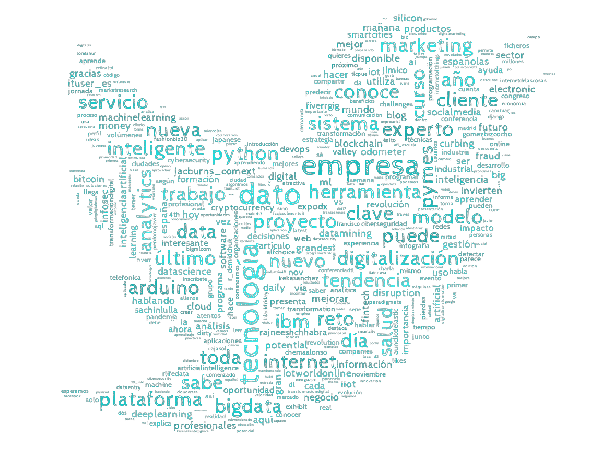
\includegraphics[scale = 1.15]{C:/DATOS/MBIT/Proyecto/MBITProject_Data4all/Python/images/twitter_worldcloud.png}%
\figcaption{Texto de los tuits}
\label{fig:twitter_worldcloud} }



\subsubsection{Tuits originales frente a tuits retuiteados}
Nos interesaba saber qué proporción de tuits de los que hemos bajado son tuits originales
y qué proporción son tuits retuiteados. En general, en los documentos obtenidos a través
del API Streaming, Twitter marca con un \lq\lq RT\rq\rq
al comienzo del texto del tuit aquellos que son retuiteados, a la vez que incluye en el cuerpo del
tuit la información completa sobre el tuit que ha sido retuiteado.Hemos observado
que hay tuits que parece que son retuits de otros (que comienzan por  \lq\lq RT\rq\rq), pero luego
no tienen los campos \lq\lq retweeted\_status\rq\rq o \lq\lq quoted\_status\rq\rq. Estos podrían ser mensajes procedentes
de bots, que los envían de forma automática. De los $14.736$ tuits,  hay 
$6.421$ originales, $8.048$ retweets estándar y $267$ aparentes retuits que no tienen información
de lo retuiteado.

\myfigure{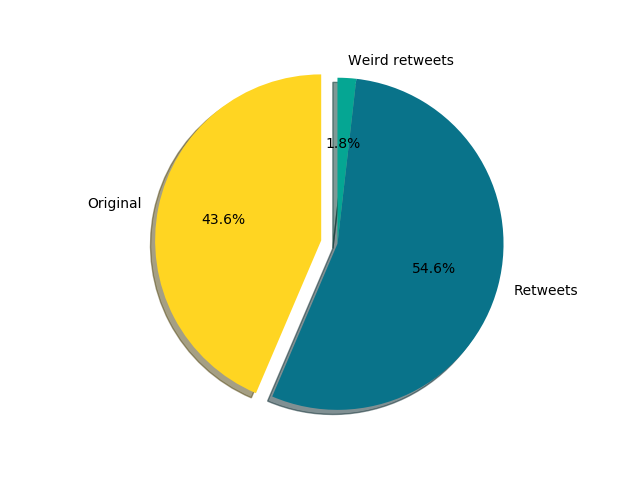
\includegraphics[width=0.6\textwidth]{C:/DATOS/MBIT/Proyecto/MBITProject_Data4all/Python/images/retweeted_proportions.png}%
\figcaption{Proporción de tuits originales y retuiteados.}
\label{fig:tuits_originales_y_retuiteados} }

\subsubsection{Número de retuits por tuit}
A la vista del gráfico anterior, parece que la actividad principal que hemos captado es
una actividad de difusión, en la que los usuarios retuitean información de otros usuarios.
Entre estos tuits retuiteados, nos interesa estudiar el número de veces que 
cada tuit ha sido retuiteado. Nos vamos a fijar en aquellos tuits que aparecen como retuiteados en nuestra muestra, es decir, aquellos tuits cuya información viene en los campos \lq\lq retweeted\_status\rq\rq o \lq\lq quoted\_status\rq\rq,
ya que son indicativos de los temas que interesan a los usuarios.
En los $8.048$ tuits de nuestro corpus que son retuits con info de lo retuiteado, se han retuiteado $2.686$ tuits distintos. La distribución del número de retuits por cada uno de estos $2.686$ aparece en las siguientes
gráficas.

\myfigure{
\begin{tabular}{cc}
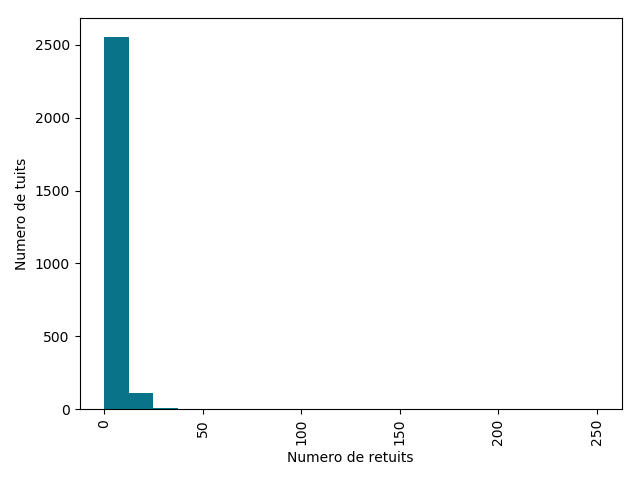
\includegraphics[width=0.4\textwidth]{C:/DATOS/MBIT/Proyecto/MBITProject_Data4all/Python/images/retweeted_graph_hist.png}
&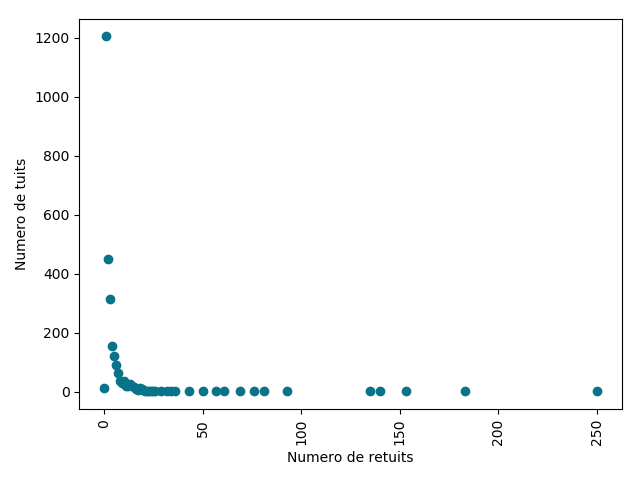
\includegraphics[width=0.4\textwidth]{C:/DATOS/MBIT/Proyecto/MBITProject_Data4all/Python/images/retweeted_graph_scatter.png}
\end{tabular}
\figcaption{Retuits: número de retuits por tuit.}
\label{fig:numero_retuits_por_tuit} }

Tanto en el histograma con en el gráfico de puntos, es claro que la mayoría de tuits han sido retuiteados unas pocas
veces (entre 1 y 5), y que solo unos pocos han sido retuiteados muchas veces. Los dos más tuiteados aparecen en la siguiente figura:

\myfigure{
\begin{tabular}{cc}

\includegraphics[width=0.4\textwidth]{tuit_mas_retuiteado}
&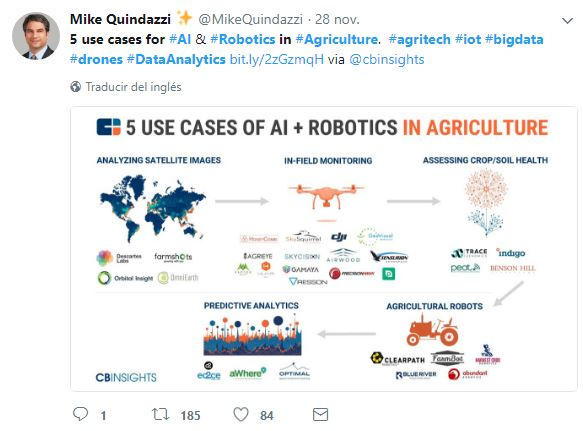
\includegraphics[width=0.4\textwidth]{tuit_mas_retuiteado2}
\end{tabular}
\figcaption{Retuits: los dos tuits más retuiteados.}
\label{fig:tuit_mas_tuiteado} }

Viendo los tuits, parece que podemos encontrar usuarios relevantes para nuestro proyecto no solo en los usuarios que han publicado los tuits que hemos descargado, sino también en los usuarios que han publicado los tuits que los primeros han retuiteado.

\subsubsection{Tuits descargados a lo largo del tiempo}
Hemos descargado tuits durante dos semanas a finales de Noviembre de 2017. La distribución
temporal del número de tuits obtenidos es la siguiente:

\myfigure{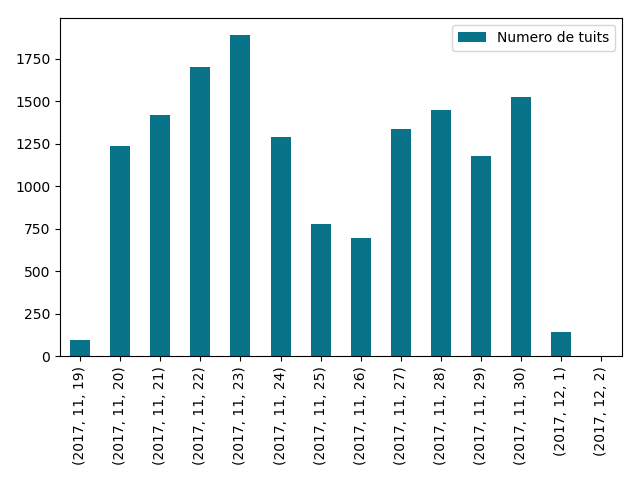
\includegraphics[width=0.6\textwidth]{C:/DATOS/MBIT/Proyecto/MBITProject_Data4all/Python/images/time_histogram.png}%
\figcaption{Tuits descargados diariamente.}
\label{fig:tuits_descargados_diariamente}}

El día 19 de Noviembre fue domingo, parece por tanto que se aprecia cierto patrón estacional en la actividad
(tuiteándose más entresemana que en fin de semana). Los días 22 y 23 de Noviembre hubo un evento
BigData, el V Encuentro de Big Data en Castilla y León, que tal vez tenga relación con la mayor actividad durante esos días.

\subsubsection{Relación entre número de tuits descargados y número de usuarios distintos}
Para nuestro proyecto, lo más relevante de la base de datos con la que trabajamos es
qué información sobre los usuarios podemos extraer a partir de los tuits almacenados. El primer paso suele ser contar, y por ello miramos cuántos usuarios distintos podemos obtener de ella. 
El siguiente gráfico representa el número de usuarios distintos en función del número de tuits
descargados, a lo largo del tiempo.

\myfigure{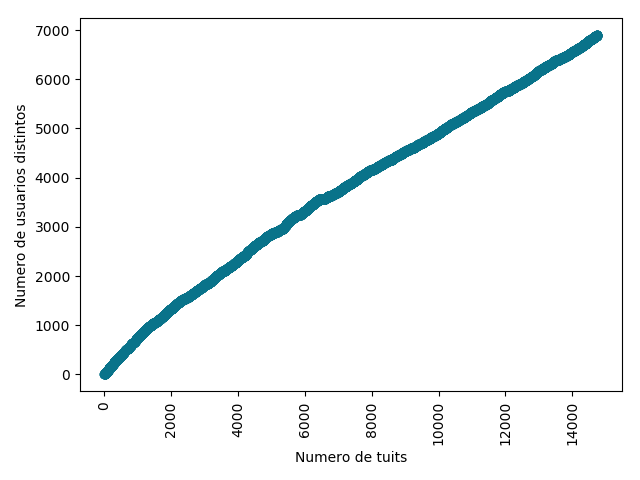
\includegraphics[width=0.6\textwidth]{C:/DATOS/MBIT/Proyecto/MBITProject_Data4all/Python/images/tuits_users_graph.png}%
\figcaption{Número de usuarios distintos frente a número de tuits descargados diariamente.}
\label{fig:tuits_users_graph}}

Este gráfico no presenta sorpresas, y se aprecia que la relación entre el número de tuits descargados y el número de usuarios distintos es prácticamente lineal.

Tenemos $6.890$ usuarios distintos (en los usuarios de los tuits descargados, sin contar los usuarios de los tuits que estos usuarios hayan podido retuitear), lo que arroja una media de unos $2.13$ tuits por usuario. Ya sabemos que la media es una medida muy poco robusta. Si queremos hacernos una idea de la actividad de nuestros usuarios, mejor estudiamos un poco más la distribución de esa variable.

\subsubsection{Número de tuits por usuario}
Al igual que hicimos con el número de retuits por tuit retuiteado, veamos un poco más en detalle
la distribución del número de tuits que cada usuario ha publicado:

\myfigure{
\begin{tabular}{cc}
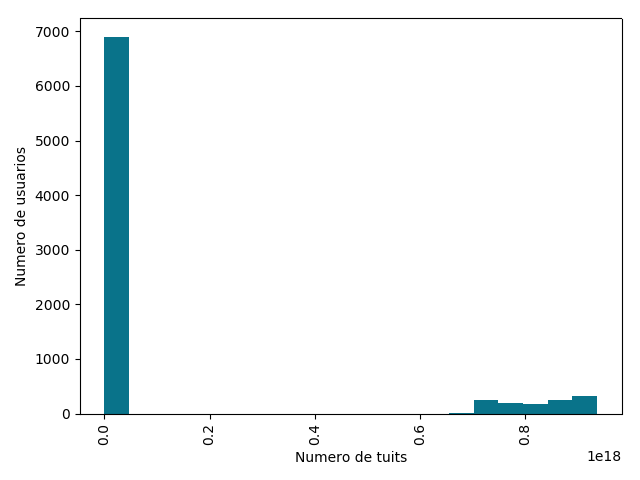
\includegraphics[width=0.4\textwidth]{C:/DATOS/MBIT/Proyecto/MBITProject_Data4all/Python/images/tuits_by_user_graph.png}
&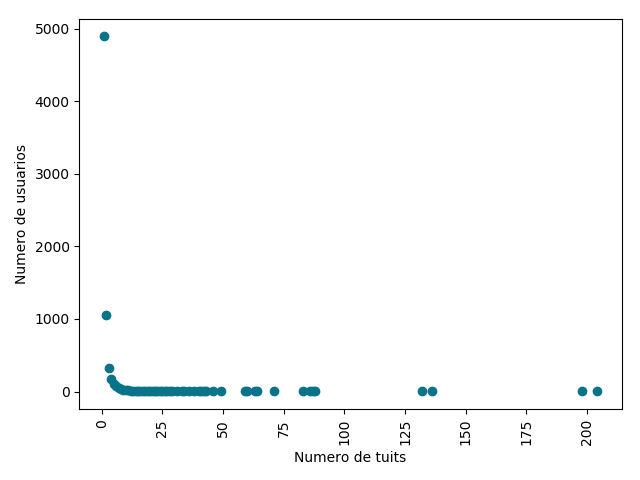
\includegraphics[width=0.4\textwidth]{C:/DATOS/MBIT/Proyecto/MBITProject_Data4all/Python/images/tuits_by_user_graph_scatter.png}
\end{tabular}
\figcaption{Número de tuits por usuario.}
\label{fig:tuits_by_user_graph_scatter} }

También en este caso se aprecia que la mayoría de los usuarios han tuiteado una vez, pero que hay algunos usuarios con un número muy elevado de tuits:

\myfigure{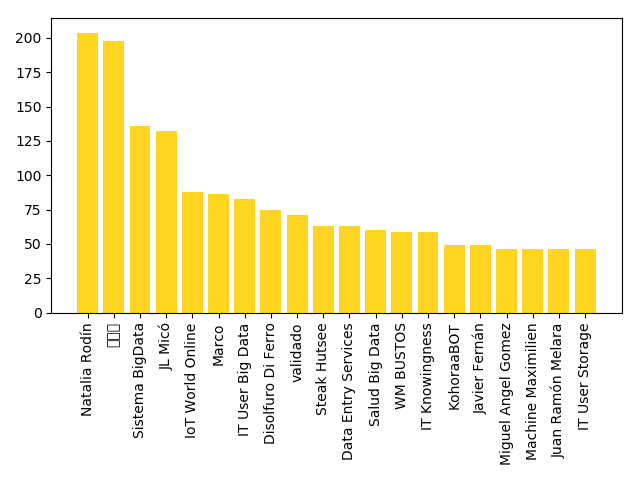
\includegraphics[width=0.6\textwidth]{C:/DATOS/MBIT/Proyecto/MBITProject_Data4all/Python/images/tuits_by_user_graph_bargraph.png}%
\figcaption{Número de tuits de los usuarios más activos.}
\label{fig:tuits_by_user_graph_bargraph}}

De estos usuarios:
\begin{itemize}
\setlength\itemsep{-0.1cm}
\item Natalia Rodín, Sistema BigData, Steak Hutsee parece que ya no existen en Twitter
\item IoT World Online es un grupo de personas interesadas en el mundo del Big Data.
\item IT User Big Data, validado, Data Entry Services, IT User Storage no está claro si son personas (solo retuits, sin bio o con bio poco descriptiva).
\item Salud Big Data es un portal de noticias
\item IT Knowingness es un feed 
\item KohoraaBot, Machine Maximilien son bots
\end{itemize}

En resumen, solo ocho de los veinte usuarios con mayor actividad parecen adecuados para
nuestro proyecto. Esto es indicativo de que la labor de filtrado de la base de datos
va a ser clave para conseguir un producto exitoso.

\subsubsection{Localización de los tuits}
Desde el punto de vista de la comercialización del producto, parece relevante incorporar información geográfica acerca de los candidatos. Para ello, siguiendo el enfoque de este trabajo, deberíamos usar información de este tipo extraída del corpus de tuits descargados de Twitter. Esto nos lleva a preguntarnos cuántos de ellos tienen el dato disponible. 

Según la documentación del API de Twitter\footnote{\url{https://developer.twitter.com/en/docs/tweets/data-dictionary/overview/geo-objects }},
los tuits pueden asociarse con una localización, generando un tuit que ha sido \lq\lq geolocalizado\rq\rq, y estas localizaciones pueden ser un punto exacto (con coordinadas de longitud y latitud) o un lugar como una ciudad o país o un área definida mediante una \lq\lq bounding box\rq\rq. Hay dos campos en un tuit que se usan para describir la geolocalización: \lq\lq coordinates\rq\rq y \lq\lq place\rq\rq. El objeto \lq\lq place\rq\rq siempre está presente en el caso de que el tuit esté geolocalizado, mientras que las coordinadas solo en el caso en el que el tuit tenga asignada una localización exacta. En el siguiente gráfico hemos 
representado el porcentaje de tuits con el campo \lq\lq place\rq\rq con valores, en el que
podemos apreciar que, salvo que cambiásemos la búsqueda en Twitter, no es un campo que vayamos a poder usar en el análisis:

\myfigure{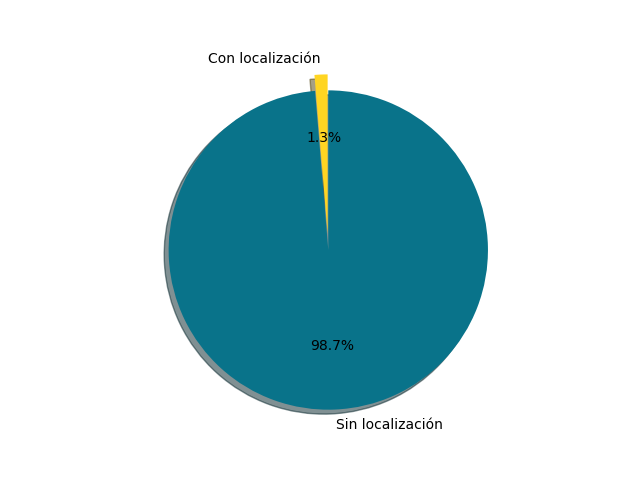
\includegraphics[width=0.6\textwidth]{C:/DATOS/MBIT/Proyecto/MBITProject_Data4all/Python/images/geolocalized_proportions.png}%
\figcaption{Proporción de tuits geolocalizados.}
\label{fig:geolocalized_proportions}}



\subsubsection{Hashtags: distribución}
En nuestro proyecto, va a ser muy importante cómo clasifiquemos los contenidos de los tuits. 
Los propios usuarios clasifican los contenidos de los tuits cuando los etiquetan a través
de los denominados \lq\lq hashtags\rq\rq,  que son palabras precedidas por el símbolo \# 
(almohadilla o {\em hash}).

Hemos estudiado los hashtags incluidos en los tuits de la base de datos, tanto los de los tuits
descargados, como de aquellos citados o retuiteados en ellos. Los siguientes gráficos dan una idea de los hashtags presentes en ambos casos:

\myfigure{
\begin{tabular}{c}

\includegraphics[width=\textwidth]{C:/DATOS/MBIT/Proyecto/MBITProject_Data4all/Python/images/hashtags_host_wordcloud.png}\\
\vspace{-1cm}\\
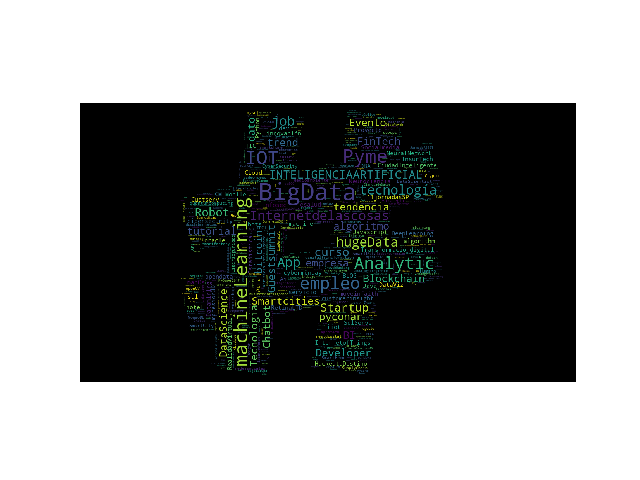
\includegraphics[width=\textwidth]{C:/DATOS/MBIT/Proyecto/MBITProject_Data4all/Python/images/hashtags_total_wordcloud.png}\\
\end{tabular}
\figcaption{Hashtags en los tuits descargados (arriba) y en los tuits descargados y citados y retuiteados en ellos.}
\label{fig:hashtags_wordcloud} }

En principio parece que no difieren mucho. Vamos a comparar los hashtags más frecuentes
en ambos conjuntos de tuits:

\myfigure{
\begin{tabular}{cc}
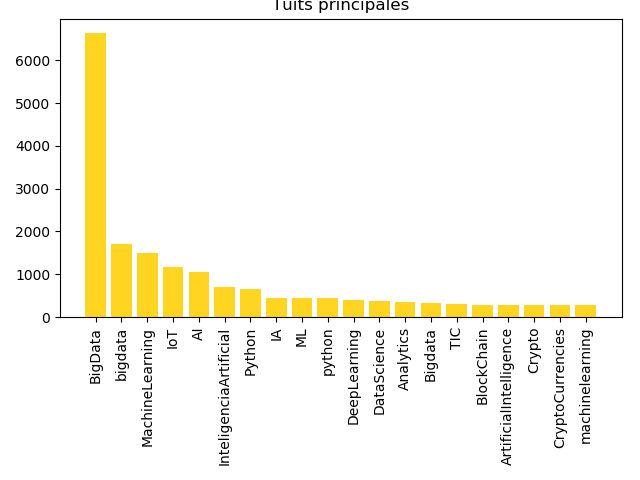
\includegraphics[width=0.4\textwidth]{C:/DATOS/MBIT/Proyecto/MBITProject_Data4all/Python/images/hashtags_host_occurs.png}
&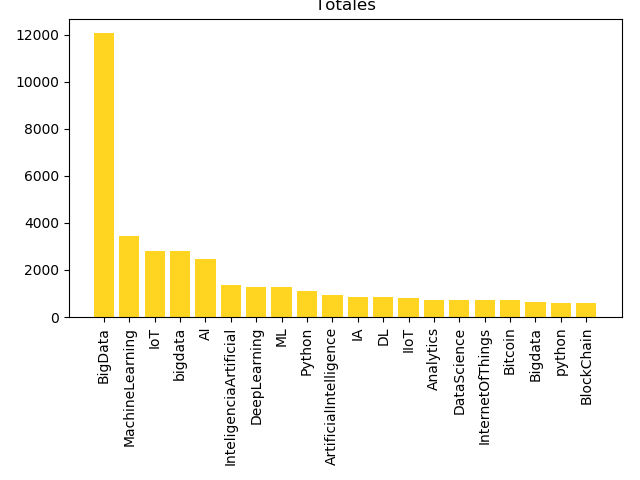
\includegraphics[width=0.4\textwidth]{C:/DATOS/MBIT/Proyecto/MBITProject_Data4all/Python/images/hashtags_total_occurs.png}
\end{tabular}
\figcaption{Hashtags más frecuentes en los tuits descargados (izq.) y en los tuits descargados y citados y retuiteados en ellos.}
\label{fig:hashtags_occurs} }

\subsubsection{Perfiles de los usuarios}
A la hora de desarrollar el proyecto y construir la lista de usuarios recomendados, es importante
filtrar aquellos que sean efectivamente personas, y desechar aquellos que sean empresas, bots, cuentas
oficiales de organismos públicos, etc.

Este análisis lo llevaremos a cabo usando la información contenida en el campo \lq\lq user\rq\rq
de los tuits, y será necesario para ello examinar el texto de la bio que incorpora, campo que
registra la información que los propios usuarios facilitan sobre ellos mismos. 
Para hacernos una idea del tipo de texto y contenidos a los que nos enfrentamos, hemos dibujado también
una nube de palabras que represente esta información.


\myfigure{

\includegraphics[width=\textwidth]{C:/DATOS/MBIT/Proyecto/MBITProject_Data4all/Python/images/bios_worldcloud2.png}
\figcaption{Wordcloud de las descripciones de los usuarios.}
\label{fig:bios_worldcloud2} }

\myfigure{
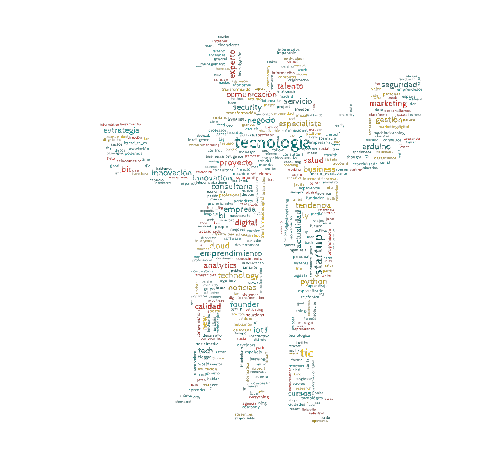
\includegraphics[width=\textwidth]{C:/DATOS/MBIT/Proyecto/MBITProject_Data4all/Python/images/bios_worldcloud.png}
\figcaption{Wordcloud de las descripciones de los usuarios.}
\label{fig:bios_worldcloud}}

Aparentemente, las descripciones de los usuarios coinciden con los perfiles que nos interesan.



\chapter{Limpieza de datos: extracción de usuarios relevantes}
\label{chap:extraccion_de_usuarios}

Como hemos visto en el análisis exploratorio inicial de los datos, la fase 
de limpieza de la información va a ser muy relevante para conseguir
nuestro objetivo final. Se trata de extraer, a partir de los tuits almacenados, 
una lista de usuarios que pudieran constituirse en candidatos adecuados a 
una oferta de trabajo (como, por ejemplo, las de la figura \ref{fig:ofertas_descripcion}). 
Para ello, de todos aquellos usuarios de los que tenemos constancia en 
los tuits recogidos hemos de seleccionar aquellos que sean personas (eliminando bots, 
empresas, etc.) y que hayan publicado contenido relacionado con la materia de referencia, 
en este caso la ciencia de datos.


Los desarrollos descritos en este capítulo están en el fichero {\bf user_selection.py}, 
que puede encontrarse en el repositorio de GitHub.

\section{Detección del idioma} 

El primer paso para poder analizar el contenido de un tuit y determinar si dicho tuit 
(y por tanto el usuario que lo ha publicado) está relacionado con la ciencia de datos o el big data,
es determinar el lenguaje en el que está escrito. Como ya hemos mencionado,
aunque la búsqueda en Twitter se realizó solicitando el campo \lq\lq languages = ["es"]\rq\rq,
obtenemos algunos tuits en otros idiomas, como estos dos 
que mostramos a continuación:

\myfigure{
\begin{tabular}{cc}

\includegraphics[width=0.4\textwidth]{tuit_ingles1}
&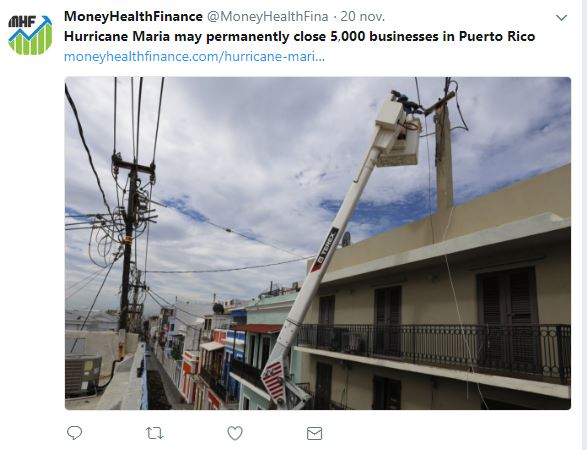
\includegraphics[width=0.4\textwidth]{tuit_ingles2}
\end{tabular}
\figcaption{Tuits no solo en español.}
\label{fig:tuits_ingles} }

Los primeros trabajos sobre el problema de la detección automática del lenguaje de un texto
se remontan a la década de 1970 \cite{zissman-berkling}. En la mayoría de las propuestas, 
existe una fase de entrenamiento, sobre textos previamente clasificados, en la que se produce 
un modelo del lenguaje (tal vez uno por lenguaje), y una fase de reconocimiento, en la que 
el lenguaje de mayor verosimilitud para el texto se extrae a partir de la aplicación de los 
distintos modelos. La clave de todos estos métodos es la modelización del lenguaje, algo que puede 
conseguirse atendiendo a diversas características diferenciadoras: fonemas, morfología, 
sintaxis y/o prosodia. 

La aplicación de dichas técnicas a textos provenientes de entornos web, blogs,  foros, etc. 
no está exenta de problemas, ver por ejemplo \cite{almeida_estevez_piad}.
Los textos procedentes de entornos web en general, y de Twitter en particular, 
presentan elevados niveles de lo que podríamos denominar como \lq\lq ruido\rq\rq,
por ejemplo:
\begin{itemize}
\item suelen ser textos cortos, lo que dificulta la aplicación de técnicas basadas en frecuencia 
de palabras o caracteres,
\item presencia de enlaces web, etiquetas, emoticonos y otros caracteres propios del entorno,
\item uso de jerga, lenguaje informal y palabras en idiomas distintos del principal del texto,
\item modificaciones de la ortografía, que van desde palabras abreviadas (\lq\lq q\rq\rq, 
\lq\lq xa\rq\rq) a expresiones enfáticas (\lq\lq mooooooolaaaaaaaa\rq\rq), por poner dos 
ejemplos.
\end{itemize}


A pesar de que es posible encontrar corpus de textos con estas características 
ya clasificados por 
idioma\footnote{\url{https://blog.twitter.com/engineering/en_us/a/2015/evaluating-language-identification-performance.html }}
que pudieran servir para entrenar un modelo que determinara el lenguaje,
hemos optado por usar un clasificador que no necesite entrenar un modelo, 
ya que esta parte del proyecto no es la principal. Hemos encontrado
referencias, como \cite{almeida_estevez_piad}, que apuntan al buen comportamiento de 
clasificadores que no depende de conjuntos de entrenamiento (basados en \lq\lq small words\rq\rq,
también denominadas \lq\lq stop words\rq\rq, y trigramas). Pero este método requiere de una implementación
{\em ad-hoc}, y las opciones disponibles, listas para usar, nos han parecido lo suficientemente
buenas para el objetivo que perseguimos en este apartado.


En el entorno de Python, hemos encontrado varios paquetes que tratan el 
problema de detectar el idioma de un texto automáticamente. Los más
comentados son los siguientes:
\begin{itemize} 
\item {\tt langid} \cite{langid}: es un paquete que proporciona un 
clasificador Naïve Bayes de textos, que usa $n$-gramas (secuencias de $n$ caracteres en el texto, con $1\leq n\leq 4$). 
El clasificador está pre-entrenado sobre diversos corpus de texto, en un total de 97 idiomas. Según los
resultados explicados en el artículo de presentación del trabajo, es un método con una
exactitud ({\em accuracy}) del 94\%.
\item {\tt langdetect}: de Nakatani Shuyo, también es un clasificador Naïve Bayes basado en $n$-gramas, con
normalizaciones heurísticas, \url{https://github.com/shuyo/language-detection }.
\item {\tt LDIG}: es un clasificador específico para Twitter, creado por el autor
de {\em lagdetect} para solventar las carencias de éste en la clasificación de mensajes
cortos, \url{https://github.com/shuyo/ldig }. Soporta menos idiomas que los anteriores.
\item {\tt equilid}: es el paquete de más reciente creación que hemos encontrado,
que además está especialmente diseñado para tratar el \lq\lq ruido\rq\rq
que comentábamos caracteriza los textos de Twitter. Está concebido para identificar
dialectos urbanos y tratar correctamente expresiones de jerga.
\end{itemize}

Dado el tema que nos ocupa, relacionado con ciencia de datos, la especialización 
de {\tt equilid} y la dificultad de su instalación en el sistema disponible
(usa una versión de TensorFlow que aparentemente no está desarrollada para Windows),
nos hace descartarlo de entrada. 
En \cite{langid2} se muestra que el comportamiento de cualquiera de los clasificadores 
restantes es lo suficientemente bueno por
separado para el objetivo de este proyecto. Sugieren que combinar dos o más clasificadores
puede mejorar la exactitud de la clasificación, y que en general, la limpieza de
los tuits (urls, etiquetas, menciones, etc.), si bien mínimamente en algunos casos,
suele mejorar el comportamiento de los modelos (excepto en el caso de {\tt langid}). 
Finalmente, nos hemos decidido por usar el algoritmo del paquete {\tt langid}, visto
el buen resultado reportado, y la facilidad de uso del mismo. 

En \cite{langid2} se muestra que, en un contexto general de detección del lenguaje, 
el paquete {\tt langid} no parece beneficiarse de una limpieza del tuit
para retirar urls, menciones, etiquetas y emoticonos del cuerpo del mensaje.
Sin embargo, dado que la implementación de esa limpieza no 
es difícil, hemos comparado la clasificación del lenguaje obtenido
con el texto original y con el texto limpio, y hemos observado que en los
textos de los $24,128$ tuits descargados (contando retuiteados y citados también)
hay un $6.37$\% de tuits que no tienen la misma asignación de lenguaje. 
Estos tuits suelen ser tuits con pocas palabras
o con mucha mezcla de idiomas (generalmente español e inglés).

Como método alternativo, se ha implementado un clasificador manual que solo
usa \lq\lq stop words\rq\rq para tratar esos casos en los que {\tt langid}
no da una elección clara del idioma. Si el método de los \lq\lq stop words\rq\rq
da un idioma para el texto que coincide con alguno de los proporcionados por 
{\tt langid} (bien el del texto limpio, bien el del texto original), ese será
el que se asigne al tuit. Y si no, lo dejaremos clasificado con un idioma desconocido.

Hemos aplicado este método de clasificación del lenguaje a los $24,128$ textos
de los tuits originales, retuiteados o citados, y resulta una clasificación en $25$
idiomas diferentes. Mostramos a continuación un resumen de los resultados del clasificador:


\myfigure{
\begin{tabular}{cc}
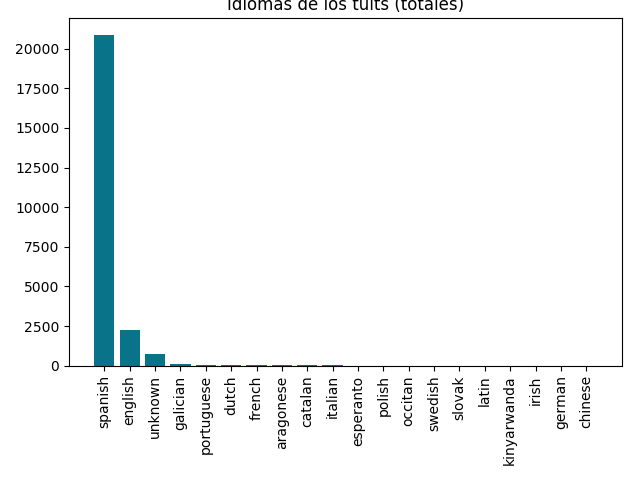
\includegraphics[width=0.4\textwidth]{C:/DATOS/MBIT/Proyecto/MBITProject_Data4all/Python/images/assigned_languages.png}
&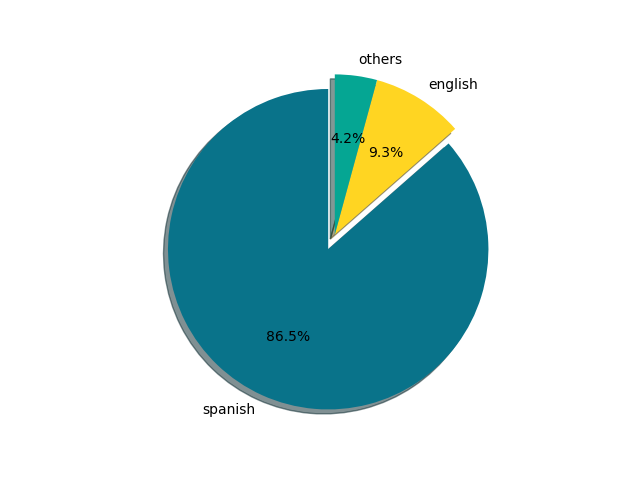
\includegraphics[width=0.4\textwidth]{C:/DATOS/MBIT/Proyecto/MBITProject_Data4all/Python/images/assigned_languages_proportions.png}
\end{tabular}
\figcaption{Clasificación por lenguaje del texto del tuit. Del $4.2$\% de \lq\lq others\rq\rq
hay un $2.9$\% de \lq\lq unknown\rq\rq. ¿Errores de clasificación?}
\label{fig:assigned_languages} }

Echando un vistazo a los resultados, aquellos que no están clasificados o que están
clasificados en idiomas poco probables, digamos, como el esperanto, son aquellos en los
que el clasificador seguramente ha fallado. Algunas veces parece ser porque casi no 
tuvieran texto o porque el texto contenga mucha mezcla de idiomas. Pero otras veces, 
como en el siguiente caso clasificado en esperanto, no está muy claro por qué:

\myfigure{
\begin{tabular}{cc}

\includegraphics[width=0.8\textwidth]{tuit_esperanto1}
\end{tabular}
\figcaption{Tuit clasificado como esperanto.}
\label{fig:tuit_esperanto1} }


\section{Tipo de usuario}
Para clasificar al usuario respecto a su entidad, y por ejemplo distinguir entre personas, bots y empresas, 
nos parece que la parte del tuit que más información contiene, a partir de los datos conseguidos, es
la bio que los propios usuarios aportan. Antes de cualquier labor de análisis de esos textos,
es necesario saber el idioma en el que están, y por ello de nuevo aplicamos a nuestros datos 
el identificador de lenguaje que usamos en el apartado anterior. 

Primero seleccionamos los datos correspondientes a los usuarios distintos, obteniendo
$7,210$ usuarios con distinto \lq\lq{\em id\_str}\rq\rq. {\tt langid} clasifica de 
forma diferente el idioma de los datos de perfil antes y después de 
limpiarlos (quitar urls, emojis, hashtags, etc.) en un $5.99$\%
de los casos. Después de aplicar en éstos últimos el método de las \lq\lq stop words\rq\rq, 
los perfiles de los usuarios han quedado clasificados en $44$ idiomas diferentes.

\myfigure{
\begin{tabular}{cc}
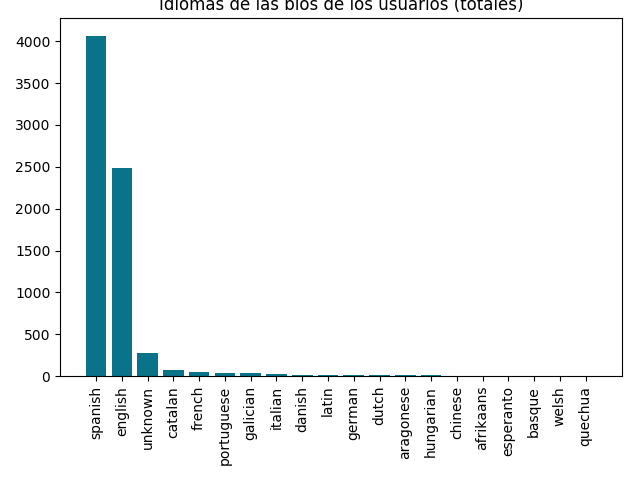
\includegraphics[width=0.4\textwidth]{C:/DATOS/MBIT/Proyecto/MBITProject_Data4all/Python/images/user_bios_assigned_languages.png}
&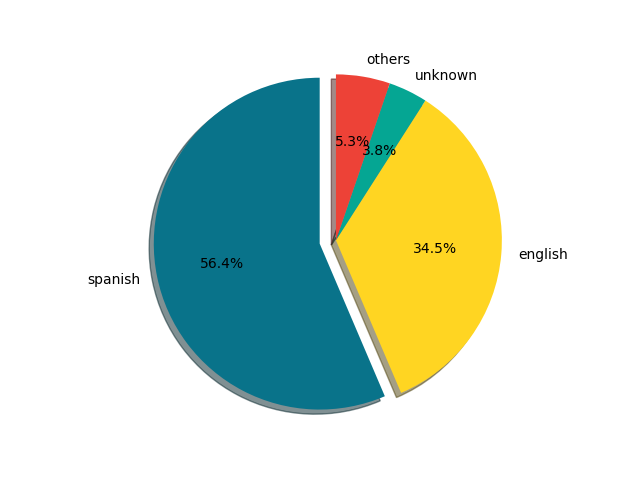
\includegraphics[width=0.4\textwidth]{C:/DATOS/MBIT/Proyecto/MBITProject_Data4all/Python/images/user_bios_assigned_languages_proportions.png}
\end{tabular}
\figcaption{Clasificación por lenguaje del texto de las bios.}
\label{fig:user_bios_assigned_languages} }


\section{Naturaleza del tuit}
texto del tuit:  IT, cientifico, analista o nodatascience (diccionarios de palabras)
					/Binario, data science o no data science

\chapter{Modelado de los datos: ordenación de los usuarios}
\label{chap:ordenacion_de_usuarios}

Una vez que ya tenemos una lista de usuarios cuyas publicaciones en Twitter
indican que podrían ser candidatos para las ofertas de trabajo, el siguiente
paso es ordenarlos de acuerdo a su relevancia. A continuación describimos brevemente
los dos criterios que usaremos para ordenarlos (el detalle de los algoritmos y 
procedimientos llevados a cabo en cada caso se hará en la secciones siguientes):
\begin{itemize}
\item Ordenación de tipo índice $h$. El índice h es un sistema propuesto por Jorge Hirsch, de la Universidad de California, para la medición de la calidad profesional de los científicos, en función de la cantidad de citas que han recibido sus artículos científicos\footnote{\url{https://en.wikipedia.org/wiki/H-index }}. Un científico tiene índice $h$ si ha publicado $h$ trabajos con al menos $h$ citas cada uno. El índice se diseñó para medir eficazmente la calidad del investigador, a diferencia de sistemas de medición más sencillos que cuentan citas o publicaciones, donde se hace una distinción entre aquellos investigadores que tienen una gran influencia en el mundo científico de aquellos que simplemente publican muchos trabajos. En nuestro campo, lo que queremos es medir 
la relevancia de los candidatos, así que una métrica de este tipo aplicada a los tuits publicados
de la temática de interés (Big Data y ciencia de datos en nuestro caso), nos ayudará a determinarla.
Los detalles, en la sección \ref{subsect:indice_h}.

\item Ordenación en función del papel de cada usuario dentro de la red de usuarios
seleccionados (sección \ref{subsect:grafo}). Para ello, construiremos el grafo 
de los candidatos y sus relaciones, siendo estas relaciones dirigidas (A está relacionado
con B si A sigue a B).
\end{itemize}

Con estos dos métodos pensamos que quedará bastante bien representado el panorama
de candidatos a partir de la información extraída de Twitter. 
Todos los cálculos descritos en esta parte del proyecto están en el archivo
{\bf user\_rank.py} del repositorio de GitHub.

En las siguientes secciones detallamos los algoritmos que hemos usado para cada sistema de
clasificación, aportando la justificación de las diversas elecciones que 
hemos llevado a cabo.

\section{Índice h}
\label{subsect:indice_h}
La particularización del índice $h$ a nuestro contexto podría ser 
del siguiente modo: un usuario de Twitter tendrá índice $h$ si $h$ de sus $N$ tuits
sobre un determinado tema, han sido retuiteados al menos $h$ veces.

Calcular el índice $h$ implica por tanto los siguientes pasos:
\begin{enumerate}
\item Explorar el timeline\footnote{\lq\lq Timeline\rq\rq es la palabra
que usan en Twitter para referirse a un flujo de publicaciones a lo largo del tiempo.
El timeline de un usuario es el flujo de las publicaciones de ese usuario.} 
de cada usuario. Para ello usaremos la función
{\tt user\_timeline} que ofrece el paquete de Python {\tt Tweepy}. 
\item Determinar, dentro de ese timeline, qué tuits son del tema que nos interesa
(Big Data o ciencia de datos) y descartar el resto.
\item De cada tuit publicado sobre el tema de interés, anotar su número de 
retuits y calcular el índice $h$. 
\end{enumerate}

La descarga del timeline de usuarios tienen varias limitaciones en el acceso a través 
del API de Twitter\footnote{\url{https://developer.twitter.com/en/docs/tweets/timelines/api-reference/get-statuses-user_timeline }}:
\begin{itemize} 
\item límite de $1500$ llamadas por cada ventana de $15$ minutos,
\item solo se permite acceder a los $3200$ más recientes tuits de cada usuario,
\item el número de tuits descargados en cada llamada al API solo puede ascender a $200$.
\end{itemize}
Para que el proceso de obtención de datos no se pare cuando alcanzamos el límite
de llamadas (da un error), la función de {\tt Tweepy} permite incluir el parámetro 
{\tt wait\_on\_rate\_limit = True} para gestionar ese error y esperar a reanudar
el proceso cuando sea posible.

La función del API de Twitter para obtener el timeline de los usuarios no tiene 
la opción de buscar tuits de forma temporal (por ejemplo, los de los tres
últimos meses). Hemos optado por evaluar el timeline respecto a los últimos
$200$ tuits publicados por parecernos un número lo suficientemente amplio para 
el objetivo de clasificar los usuarios, si bien se podría incluir en el código la
gestión de un número mayor de tuits en el timeline (aumentando el número de
llamadas al API).

Un aspecto importante a la hora de evaluar el impacto del usuario es distinguir 
entre sus publicaciones originales y los retuits. De los tuits que componen el 
timeline, vamos a extraer la siguiente información:
\begin{itemize}
\item el número de tuits descargados(que 
en principio serán $200$, pero podrían ser menos),
\item el número de tuits sobre el tema de interés, y por tanto el
porcentaje de tuits de interés sobre el total de tuits evaluados,
\item sobre los tuits de interés, el porcentaje de aquellos que son retuits,
\item el índice $h$ de los tuits originales. Para calcular el índice $h$ 
contaremos tanto las veces que se ha retuiteado el tuit como las que ha sido
citado.
\end{itemize}

Como información adicional también obtendremos el idioma en el que los usuarios han 
publicado los tuits. En esta parte del proyecto reutilizamos por tanto dos herramientas
mencionadas en la parte de selección de usuarios: el modelo que nos permite detectar si
un tuit es relevante o no (explicado en la sección \ref{sect:tuits_relevantes})
y el algoritmo para detectar el idioma de un texto (visto en la sección \ref{sect:deteccion_idioma}).

Al intentar bajar el timeline de algunos usuarios se pueden
obtener diversos mensajes de error (por ejemplo, porque el usuario tenga
protegido su timeline, porque el usuario haya dejado de existir, etc.)
de forma que el proceso puede fallar. El código debe contemplar ese
caso y permitir que la ejecución continue con el resto de usuarios:

\myfigure{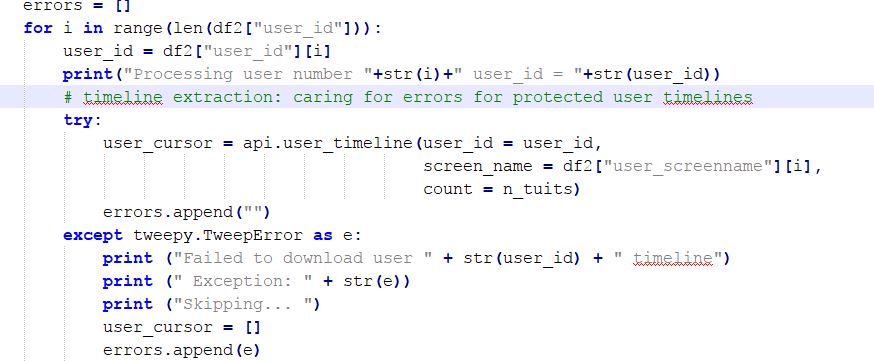
\includegraphics[width=0.6\textwidth]{error_not_authorized}%
\figcaption{Control de errores en la descarga de timelines.}
\label{fig:error_not_authorized} }

Una vez obtenidos los tuits relevantes del timeline de cada usuario, y
el número de veces que han sido retuiteados, la función que calcula el índice
$h$ es la siguiente:

\myfigure{\includegraphics[width=0.6\textwidth]{h_index_function}%
\figcaption{Función para el cálculo del índice $h$.}
\label{fig:h_index_function} }

\section{Grafo relacional}
\label{subsect:grafo}
Nuestro objetivo en esta parte es explorar las relaciones entre los usuarios que 
hemos identificado como relevantes. De forma natural, como en cualquier red social,
se pueden definir multitud de estructuras de tipo grafo para describirlas. Nosotros
vamos a usar un grafo cuyos vértices serán los usuarios, y cuyas aristas o arcos serán
las relaciones entre ellos, de tipo dirigido: el usuario A está relacionado con el
usuario B si A sigue a B (y puede muy bien ocurrir que B no esté relacionado con A,
según esta definición). 

Para esta parte necesitaremos entonces descargar de Twitter la información
necesaria para construir el grafo de relaciones: los seguidores 
(\lq\lq followers\rq\rq\footnote{A aquellos usuarios que siguen a un determinado usuario, 
en Twitter se les denomina \lq\lq followers\rq\rq. Y se llaman \lq\lq friends\rq\rq aquellos
a los que dicho usuario determinado sigue.})
de cada uno de los usuarios identificados como potenciales candidatos. 
En principio, podríamos usar tanto los followers como los friends de cada uno 
de los usuarios de nuestra lista. Pero en realidad no hace falta, ya que si el usuario
A es un friend del usuario B, B es un follower del usario A, y lo consideraremos al
estudiar los followers de A. 

Para explorar los followers de cada usuario seleccionado usaremos la función 
{\tt followers\_ids} del paquete {\tt Tweepy}. Esta función es una interfaz
para la función del API de Twitter que permiten acceder a la lista de 
followers. Esta función del API de Twitter
tiene una limitación de $15$ llamadas al API por cada ventana de $15$ 
minutos\footnote{\url{https://developer.twitter.com/en/docs/accounts-and-users/follow-search-get-users/api-reference/get-followers-ids }},
con lo que la gestión de los límites es especialmente importante en este caso.
El parámetro {\tt wait\_on\_rate\_limit = True} al crear el acceso al API a 
través de {\tt Tweepy} también nos va a ser de utilidad.

Por otro lado, la información que puede descargarse con esa función también
está limitada en cantidad: el número de followers que puede obtenerse en cada llamada 
al API es a lo sumo $5000$. Igual que antes,
usando un código con varias llamadas al API, podríamos obtener un número más elevado de 
seguidores.

Nuestro grafo será por tanto un par ordenado 
$G=(N,g)$, donde $N$ es un conjunto de vértices o nodos, que serán los usuarios
identificados como potenciales candidatos para la oferta de trabajo, y $g$
es un conjunto de aristas o arcos, descritos como pares de nodos ordenados:
$$g=\{(a,b): a,b\in N, a \mbox{ sigue a }b\}.$$
En las representaciones de un grafo dirigido, una relación $(a,b)$ se 
suele describir con una flecha que sale de $a$ y apunta a $b$.
Al extraer la información sobre los usuarios hemos de quedarnos con los followers
de cada uno que están en el conjunto de usuarios, es decir, solo nos quedamos con
las relaciones entre candidatos:

\myfigure{\includegraphics[width=0.8\textwidth]{followers_code}%
\figcaption{Followers y relación entre usuarios.}
\label{fig:followers_code} }

Una vez obtenidas estas relaciones, vamos a necesitar una librería 
para procesar el grafo y sacar las pertinentes 
conclusiones. A este respecto, tenemos varias opciones que 
considerar. Entre otras:
\begin{itemize}
\item {\tt Graph-tool}: los algoritmos están implementadas en una librería C++, 
lo que aporta mucha rapidez en la ejecución. Es 
buena procesando grafos grandes. La instalación en entornos Windows no
está soportada\footnote{\url{https://git.skewed.de/count0/graph-tool/wikis/installation-instructions 
}}.
\item {\tt NetworkX} es fácil de usar, para conjuntos de datos pequeños. Está bien
documentado. Es compatible con Python 2.7, 3.4, 3.5 y 3.6.
\item {\tt SNAP} (Stanford Network Analysis Platform): es un sistema para el análisis
y la manipulación de grandes redes. Está implementada en C++, con una interfaz en Python. 
Disponible para Python 2.7\footnote{\url{https://snap.stanford.edu/snappy/index.html }}.
\item {\tt igraph}: es una colección de herramientas para análisis de grafos,
con interfaces en R, Python y C/C++. Compatible con Python 2.6, 2.7 y 3.2.
\item {\tt APGL} (Another Python Graph Library): es una librería sencilla
para procesar grafos, disponible en principio para Python 2.7\footnote{\url{https://pythonhosted.org/apgl/ }}.
\end{itemize}

Vistas las opciones, nos hemos decidido por usar {\tt NetworkX}.
Esta herramienta nos va a permitir calcular varias métricas
que usaremos para estudiar el papel de cada usuario dentro de la red
y medir su relevancia (\cite{notas_fernando}, 
\url{https://www.sci.unich.it/~francesc/teaching/network/ }), y también explorar la estructura de la red, como exponemos a continuación.

\subsection{El papel de los usuarios: medidas de centralidad}

Las medidas de centralidad de los nodos de un grafo tratan de responder a la
cuestión de cuáles son los vértices más importantes o centrales dentro del 
grafo. La \lq\lq importancia\rq\rq de un nodo puede ser entendida 
de múltiples formas, y en consonancia hay diversas medidas de la misma.

Una vez que hemos determinado la medida de centralidad que nos interese para los nodos,
podremos usarla para ordenar la lista de los nodos (que es nuestro objetivo principal).
Todas las medidas de centralidad que vamos a describir
a continuación se pueden calcular con las funciones que proporciona el
paquete {\tt NetworkX}.

\subsubsection{Centralidad por grado}
El grado (degree) de un nodo $n$ es el número de aristas 
incidentes en $n$. En los grafos dirigidos podemos distinguir entre in-degree (número
de aristas que apuntan a $n$, en nuestro caso el número de followers) y
out-degree (número de aristas que parten de $n$, en nuestro caso, el número de
usuarios a los que sigue $n$). El in-degree representaría la capacidad de 
\lq\lq liderazgo\rq\rq
del usuario (a más followers, en principio más liderazgo), y el out-degree 
representaría el interés del usuario en seguir a otros usuarios, que podríamos
interpretar como su interés por el clima general del sector.

\subsubsection{Centralidad por autovector (eigenvector centrality)}
Es una extensión del 
concepto de cen\-tra\-li\-dad por grado que captura la intuición de que la importancia 
de un nodo en la red incrementa por el hecho de estar conectado a otros nodos 
a su vez relevantes. En un grafo dirigido, como el nuestro, parece natural pensar que
es más relevante la importancia de los usuarios que siguen a uno dado,
y que por tanto deberíamos usar los enlaces que apuntan al usuario en cuestion (las 
aristas que cuentan para el in-degree) para medir su propia importancia. 

Sea $c$ el vector columna
de las centralidades por autovector de los $N$ nodos del grafo y sea $A$ la matriz $N\times N$
de adyacencia del grafo, en la que $a_{ij}$ representa la contribución
del nodo $n_i$ al \lq\lq prestigio\rq\rq del nodo $n_j$ (en nuestro caso, $a_{ij} = 1$ si
$n_i$ sigue a $n_j$ y cero en caso contrario). La idea detrás de esta centralidad
(\cite{bonacich2}) es que la centralidad de un nodo será la suma de las centralidades
de los nodos que le apuntan, ponderadas por el peso de la unión, esto es:
$$c_i = \sum_j a_{ji} c_j$$
que en notación matricial es 
$$c = A^Tc.$$
Para asegurarnos de que esta ecuación tenga solución debemos considerar una formulación más general,
en la que la centralidad no es exactamente la suma de las centralidades de los nodos que 
contribuyen, sino solo un múltiplo de dicha suma:
$$\lambda c = A^Tc,$$
de tal forma que $c$, el vector de las centralidades del grafo es un 
autovector de la matriz $A^T$. Si $A$ es una matriz $N\times N$ hay en general $N$ soluciones
a dicha ecuación, correspondientes a los $N$ autovalores de $A^T$. Suele considerarse
como solución el autovector correspondiente al máximo autovalor.
 
La centralidad por autovector tiene un problema cuando
alguno de los nodos no tiene enlaces que lo apunten (es decir, si alguno de los usuarios
no tuviera ningún seguidor entre los demás usuarios, aunque él sí que siguiera a otros),
ya que en ese caso un nodo así siempre contribuirá cero, y por tanto, en algunos casos
la centralidad por autovector de todos los nodos sería cero:

\myfigure{\includegraphics[width=0.6\textwidth]{grafos_bonacich}%
\figcaption{En los grafos I y II de estos ejemplos (extraídos de la página
192 de \cite{bonacich}), la centralidad por autovector de todos los nodos
es $0$.}
\label{fig:grafos_bonacich} }

Una medida de centralidad que puede ayudar en este tipo de situaciones es la 
centralidad de Bonacich.

% Dos medidas de centralidad que pueden ayudar en este tipo de situaciones son la 
% centralidad de Bonacich y la de Kleinberg.

\subsubsection{Centralidad de Bonacich}
Para paliar el problema mencionado anteriormente de la centralidad por 
autovector, podemos usar la centralidad de Bonacich, que  parte de la siguiente
idea: todos los nodos tienen una centralidad mínima. Con la misma notación que en el apartado
anterior, la centralidad de Bonacich puede definirse 
(ecuación $(5)$ en \cite{bonacich}) como:
$$c_i = e_i + \alpha\sum_j a_{ji} c_j, \mbox{ que en notación matricial es } c = e + \alpha A^Tc$$
donde $\alpha\in[0,1]$ y $e$ es un vector constante. Esto es, la centralidad de cada nodo es la suma
de una centralidad mínima (o exógena, como la denominan en \cite{bonacich}) 
y de las contribuciones a la centralidad de las centralidades de los nodos que apuntan 
a dicho nodo. Esa contribución se amortigua a través del parámetro $\alpha$, 
ya que para nodos a distancia $k$ de un nodo dado, su contribución es múltiplo de
$\alpha^k$. Si $\alpha=0$, no hay transmisión de centralidad.

% \subsubsection{Centralidad de Kleinberg}
% Hasta ahora, un nodo es importante si apuntan hacia él muchos nodos o si los nodos 
% que apuntan hacia él son importantes. Los nodos sin otros  nodos que apunten hacia 
% ellos, en el mejor de los casos cuentan
% con una centralidad mínima. Sin embargo, uno podría pensar que si un nodo apunta a otros nodos
% importantes, eso también debería ser importante. Por ejemplo, un artículo que cita a otros
% artículos importantes tiene el valor de indicarnos dónde encontrar información relevante y fiable.

% Podríamos entonces definir dos tipos de nodos: las autoridades (que contienen la información fiable)
% y los \lq\lq hubs\rq\rq, que nos dicen dónde está esa información fiable. La tesis de
% Kleinberg expuesta en \cite{kleinberg} es que un nodo es una autoridad si hacia él apuntan hubs,
% y es un hub si apunta hacia autoridades.

% La centralidad de Kleinberg también puede modificarse para incorporar una 
% centralidad exógena (como en la centralidad de Bonacich) o normalizar las centralidades
% de los nodos por su out-degree como en el PageRank.

% Sean $x$ e $y$ los vectores columna que denotan la centralidad por autoridad y por hub de
% los $N$ nodos del grafo. Con la misma notación que en los apartados anteriores, 
% se define la centralidad por autoridad $x_{i}$ como 
% $$x_i = \alpha  \sum_j a_{ji} \, y_j, \mbox{ o, en notación matricial, }x=\alpha  A^Ty,$$
% y la centralidad por hub como 
% $$y_i = \beta \sum_k a_{ij} \, x_j, \mbox{ esto es, } y =\beta A x,$$
% donde $\alpha$ y $\beta$ son dos constantes a determinar. Combinando las dos:
% \begin{eqnarray*}
% x & = &\alpha\beta A^T A x \\ 
% y & = &\alpha\beta A A^T y,
% \end{eqnarray*}
% y también
% $$ A x = \alpha\beta A A^T A x.$$ 
% Observemos que la matriz de autoridad $C = A^T A$ y la matriz de hub $R = A A^T$ tienen los
% mismos autovalores y que $y$ y $A x$ son dos autovectores de de la matriz de hub
% $R = A A^T$ con el mismo autovalor $1/\alpha\beta$. Entonces,
% una vez que calculamos el vector de centralidad por autoridad $x$, como 
% un autovector de la matriz de autoridad $C=A^TA$, podemos
% calcular la centralidad por hub como $y = A x$. En particular, la centralidad por hub
% del nodo $n_i$ es la suma de las centralidades por autoridad de los nodos que apuntan a $n_i$
% \footnote{La matriz $C$ se conoce como la matriz de co-citaciones
% en bibliometría: $C_{ij}=\sum_k a_{ki} a_{kj}$ es el número predecesores
% comunes de los nodos $n_i$ y $n_j$, y $C_{ii}$ es el in-degree de $n_i$. La matriz
% $R$ se conoce como la matriz de co-referencia en bibliometría: cada elemento 
% $R_{ij}=\sum_k a_{ik} a_{jk}$ es el número de sucesores comunes de $n_i$ y $n_j$, y 
% $R_{ii}$ es el out-degree de $n_i$. Esto da una interpretación alternativa de autoridades
% y hubs: un nodo es una autoridad si es muy co-citado con otras autoridades, y un nodo es un hub 
% si co-referencia a otros hubs.}.

\subsubsection{PageRank}
En las centralidades por autovector y de Bonacich, los nodos
distribuyen de forma indiscriminada su centralidad a todos los demás nodos a los que apunten, 
por lo que un nodo importante que apunta a muchos vecinos hace importantes a 
todos ellos. La idea de PageRank es repartir la centralidad aportada 
por un nodo entre todos aquellos a los que apunta, de tal forma que cada uno de ellos
recibirá solo la parte proporcional de la centralidad del nodo de partida, esto es,
la centralidad del nodo dividida por su out-degree (número de enlaces salientes):
$$c_i = (1-d) + d\sum_j a_{ji} \frac{c_j}{od(n_j)},$$
donde $od(n_j)$ es el out-degree del nodo $n_j$, y $d$ es un factor de amortiguación 
que tiene un valor entre 0 y 1. En la aplicación que hace Google de este algoritmo
(tienen una patente sobre él), parece que $d=0.85$, aunque la 
implementación concreta del algoritmo es por supuesto secreta. El papel de
$d$ es similar al de $\alpha$ en la centralidad de Bonacich, en
cuanto a la transmisión de la centralidad, y además ayuda a la convergencia
del cálculo del PageRank (se resuelve de forma iterativa).
En \cite{fdez} se puede encontrar una deliciosa explicación del algoritmo.

\subsubsection{Cercanía (closedness centrality)}
En un grafo conexo, la cercanía 
de un nodo es el inverso de la suma de las longitudes
de los caminos mínimos que unen dicho nodo con todos los demás:
$$c_i=\frac {1}{\sum _{j}d(n_j,n_i)},$$
donde $d(n_j,n_i)$ es la distancia geodésica\footnote{Las geodésicas son el camino
más corto entre dos puntos y no son necesariamente únicas.} 
entre los nodos $n_j$ y $n_i$. 

Cuanto más central es un nodo,
más cerca está del resto de nodos. Tales vértices pueden tener mejor acceso
a la información de otros nodos, o una influencia más directa en ellos. Por ejemplo, una persona
con mayor cercanía puede ver cómo sus opiniones alcanzan a otros usuarios más deprisa que 
las de alguien con menor cercanía. 

Frecuentemente, en lugar de la suma se considera la media de los caminos más cortos, 
de tal forma que se pueden comparar grafos de diferentes tamaños. Entonces, la formulación es:
$$c_i=\frac {N-1}{\sum _{j\neq i}d(n_j,n_i)},$$
donde $N$ es el número de nodos en el grafo. Si el grafo es muy grande, 
$N$ y $N-1$ son muy parecidos y suele usarse:  
$$c_i=\frac {N}{\sum _{j}d(n_j,n_i)}.$$
Considerar las distancias a o desde los otros nodos es irrelevante en grafos no dirigidos.
Pero en el caso de grafos dirigidos, puede producir resultados totalmente diferentes.
Cuando el grafo no es conexo, se puede usar la suma de los inversos de las distancias
en lugar del inverso de la suma de las distancias, con la convención 
$1/\infty =0$:
$$c_i=\sum _{j\neq i}\frac {1}{d(n_j,n_i)}.$$

\subsubsection{Intermediación (betweenness centrality)}
Captura en qué medida un nodo esta situado 
en los caminos que unen a otros nodos. Los nodos con una intermediación alta
pueden tener mucha influencia en la red, dado que \lq\lq controlan\rq\rq la información
que se transmite entre otros nodos. También son nodos que si desaparecieran impedirían
la transmisión de la información y aumentaría la desconexión de la red.

Matemáticamente, sea $n_{k,j}$ el número total de geodésicas que van desde $n_k$ a $n_j$,
y $n_{k,j}^{i}$ el número de ellas que pasan por $n_i$. Entonces, la
intermediación del nodo $n_i$ es:
$$c_i = \sum_{k,j} w_{k,j}^{i} = \sum_{k,j} \frac{n_{k,j}^{i}}{n_{k,j}},$$
donde el cociente $w_{k,j}^{i}$ expresa lo \lq\lq en medio\rq\rq que está $n_i$ de
$n_k$ y $n_j$, y por convención $w_{k,j}^{i} = 0$ si $n_{k,j} = 0$. 

Observemos que
la definición cuenta de forma distinta los caminos de $n_k$ a $n_j$ y de $n_j$ a $n_k$ 
(importante en grafos dirigidos), aquellos que empiezan o terminan en $n_i$ ($n_k=n_i$ o $n_j=n_i$) y también aquellos en los que $n_k=n_j$. Esto atiende al hecho de que parece razonable considerar
que un vértice está en medio cuando está en un camino entre él y algún otro, ya que en esos casos, también controla el flujo de información. En cualquier caso, usar otra definición no suele 
implicar mucha diferencia, ya que en general nos interesarán los valores relativos de la medida, y no
su valor absoluto. En ese sentido, suele normalizarse por el número total de pares ordenados
del grafo ($N^2$), para que la medida nos dé un número entre $0$ y $1$.

La tabla \ref{tab:medidas_cent_significado} resume las medidas de centralidad que vamos a incluir en nuestro análisis y una pequeña idea de su significado.

\begin{center}
\begin{table}
\begin{tabular}{c|c}
{\bf Centralidad} &{\bf Descripción}\\ \hline\hline
Por grado & Conexión total del usuario con la red\\ \hline
In-degree & Número de followers\\ \hline
Out-degree & Número de seguidos\\ \hline
Por autovalor & Importancia de los seguidores\\ \hline
Bonacich & Importancia de los seguidores más centralidad mínima\\ \hline
PageRank & Importancia proporcional de los seguidores más centralidad mínima\\ \hline
Cercanía & Facilidad de acceso a otros usuarios\\ \hline
Intermediación & Influencia y conexión de la red\\ \hline
\end{tabular}
\medskip
\caption{Medidas de centralidad e idea de su significado.}
\label{tab:medidas_cent_significado}
\end{table}
\end{center}

\subsection{La estructura de la red}
La teoría de grafos también nos permite extraer información
muy interesante sobre la estructura de la red de usuarios:
hay unas ciertas características que suelen aparecer en estructuras del
tipo que nos interesa, patrones que tienen un efecto importante en cómo 
se comportan estas redes.  Esta información no es directamente 
relevante para la ordenación de los usuarios, pero nos permitirá hacernos 
una idea más clara de cómo se organiza. Veamos algunas de dichas características.

\subsubsection{Estructura del grafo}
\label{sect:estructura_grafo}
\begin{itemize}
\item Componentes conexas: una componente conexa de un grafo no dirigido es
un conjunto de nodos maximal (que no se pueden añadir más) tal que cualquier par de nodos
está conectado. Las componentes conexas son una partición del grafo (son disjuntas y
su unión es el grafo completo). En numerosos ejemplos reales, suele aparecer una gran
componente conexa (la componente gigante) que cuenta con una mayoría de los nodos (típicamente
más del $50$\%, pero no es infrecuente el $90$\%).  En los grafos dirigidos la noción de 
conectividad se complica y tenemos componentes débilmente conexas y fuertemente conexas:
	\begin{itemize}
	\item Dos nodos están en la misma componente débilmente conexa si están conectados por un camino,
	donde los caminos pueden recorrerse en cualquier sentido a lo largo de cualquier arista (esto es,
	como si el grafo fuera no dirigido).Se comporta igual que en el caso no dirigido, suele haber una
	componente gigante en la que se agrupan un alto porcentaje de los nodos.
	\item Dos nodos están en la misma componente fuertemente conexa si desde cada uno de ellos se puede
	ir al otro, a través de caminos dirigidos. Las componentes fuertemente conexas también
	forman una partición del grafo, y también se puede presentar una componente gigante,
	aunque debido a las restricciones del grafo, no suele ser tan grande. 
	\end{itemize}

\item Caminos mínimos (geodésicas)
	\begin{itemize}
	\item La excentricidad de un nodo en un grafo conexo es la mayor distancia
	geodésica entre ese nodo y cualquier otro vértice del grafo. En un grafo disconexo,
	o bien todos los nodos se definen con una excentricidad infinita, o bien se calcula 
	la excentricidad en la componente conexa a la que pertenezca el nodo. 
	\item Diámetro: la mayor distancia geodésica dentro del grafo (o componente si no es conexo). 
	Es la máxima excentricidad.
	\item Radio: la mínima distancia geodésica dentro del grafo.
	\item Longitud del camino medio: media de todos los caminos mínimos entre los 
	nodos del grafo (menos sensible a valores extremos).
	\end{itemize}
\item Distribución del grado de los nodos: del grado, out-degree o in-degree, da una idea
de lo conectada que está la red. La distribución conjunta del in y el out-degree
nos proporciona información sobre la correlación entre ambas cantidades. En muchos casos,
estas distribuciones suelen ser muy asimétricas: muchos nodos con valores bajos, y unos pocos
con valores muy altos.

\item Transitividad: Tres nodos $n_1, n_2, n_3$ tales que $n_2$ está relacionado con $n_1$ y $n_3$ forman un triángulo centrado en $n_2$.
El triángulo es cerrado si $n_1$ está relacionado con $n_3$, y abierto en caso contrario. La
transitividad mide la capacidad de la red para que los triángulos sean cerrados, esto es,
si un nodo $n_1$ está conectado
con otro nodo $n_2$, y éste con un tercero $n_3$, entonces $n_1$ también está conectado
con $n_3$.  
El coeficiente de transitividad de una red, también conocido
como coeficiente de clusterización, es el cociente entre el número de triángulos 
cerrados en la red, respecto al número de posibles triángulos. Las redes sociales
tienden a tener valores altos de transitividad\footnote{\cite{notas_fernando}, \url{https://www.sci.unich.it/~francesc/teaching/network/transitivity.html }:
por ejemplo, la transitividad de la colaboración entre autores en ciencias
de la computación es $0.24$, la de la red de colaboración entre actores
$0.2$ y la de coautores en publicaciones de física, $0.45$. Sin embargo,
la de Internet es solo $0.012$.}.
En las redes dirigidas, la transitividad se calcula como para las no dirigidas,
ignorando la dirección de las aristas.
\end{itemize}


\subsubsection{Grupos de nodos}
Desde el punto de vista de nuestra aplicación, podría ser interesante
descubrir, a través del estudio de la red, los grupos que pudieran formarse
entre usuarios. Estos grupos podrían deberse a agrupaciones de usuarios en
función de similares intereses, y detectar a través de ellos la especialización
de perfiles. Por ejemplo, es razonable pensar que alguien interesado en visualización
de datos, seguirá o será seguido por usuarios cuyo perfil también incluya un
interés en visualización de datos. 

Esta parte, sin embargo, requeriría un estudio muy detallado de la estructura
de la red, que no es el objetivo principal del proyecto.

\section{Almacenamiento}
La tabla con los usuarios y sus medidas de relevancia se obtiene como un data frame
desde el código, y para almacenarlo hemos decidido exportarlo como un fichero Excel,
concretamente el fichero {\bf Python/tables/4\_ranked\_users.xlsx} del 
repositorio de GitHub, para posteriormente poder importarlo desde R y ofrecer
una buena visualización de los datos.

Análogamente, hemos guardado en un fichero el grafo una vez construido
a partir de las relaciones entre los usuarios, {\bf Python/graph/relations\_graph.gml}.
Este fichero se puede importar también desde R y desde Gephy a efectos de visualización.

\section{Resultados}
De los $155$ usuarios que teníamos para ordenar, al intentar bajar desde Twitter los 
datos (timeline y followers) de alguno de los usuarios, se ha producido un error.
En uno de ellos, el texto del error \lq\lq Not authorized.\rq\rq, indica que
es un usuario con el timeline y resto de datos protegidos.
En otro caso, el mensaje de error al acceder a timeline,
\lq\lq [{'code': 34, 'message': 'Sorry, that page does not exist.'}]\rq\rq,
solo parece indicar que es un usuario
que no existe más en Twitter. En cualquier caso, son usuarios que no van a aparecer 
ordenados en nuestra tabla. Mejor dicho, aparecerán, pero sin un valor de ordenación (todos
los indicadores a $0$).

\subsection{Ordenación de los usuarios}
Para ver la tabla ordenada de los usuarios, lo mejor que puede hacerse es
usar el Shiny que hemos desarrollado y que describimos en el siguiente capítulo.
Podemos adelatar sin embargo un análisis descriptivo de la tabla de usuarios
(por ejemplo, importando la tabla en R):
 
\myfigure{\includegraphics[width=0.8\textwidth]{results_descriptives}%
\figcaption{Análisis descriptivo de los usuarios.}
\label{fig:results_descriptives} }

Tal vez lo más llamativo sean los valores del índice $h$. Para entenderlos un
poco mejor, veamos el histograma:

\myfigure{\includegraphics[width=0.5\textwidth]{h_index_hist}%
\figcaption{Histograma de los valores obtenidos del índice $h$.}
\label{fig:h_index_hist} }

A la vista de este gráfico, los valores obtenidos del índice $h$ son nulos en
la mayoría de los casos, y solo unos pocos individuos tienen unos valores 
del índice $h$ distintos de cero. En particular, uno de ellos tiene un valor muy alto, 11.
Es el siguiente:

\myfigure{\includegraphics[width=0.3\textwidth]{highest_h_index_person}%
\figcaption{Usuario con el índice $h$ más alto.}
\label{fig:highest_h_index_person} }

Con respecto al resto de las medidas, hemos procurado que el código nos
devuelva valores normalizados de las centralidades. Nuestra idea es no sólo ordenar
los usuarios por sus niveles individuales de cada uno de los índices, sino también
poder construir índices personalizados, asignando pesos distintos a cada uno de los 
índices, y luego combinándolos. Para ello, el siguiente paso, que se lleva a cabo en
la última fase, de visualización, es la normalización también de los niveles 
del índice $h$.

\subsection{Propiedades del grafo}
El grafo que hemos obtenido está formado por $154$ nodos (todos los usuarios, menos
aquel cuyos datos están protegidos en Twitter) y $271$ arcos.

El grafo no es fuertemente conexo, y tiene $91$ componentes fuertemente conexas.
La mayor de las componentes tiene $35$ nodos, que son el $22.73$\% del total.
Se trata de un grafo bastante desconectado. No es ninguna sorpresa, ya que 
estamos buscando las conexiones entre los usuarios que hemos seleccionado 
a través de las fases que hemos detallado a lo largo de esta memoria.

Para la componente conexa de mayor tamaño, las medidas 
relevantes son las siguientes (recordar que en la sección \ref{sect:estructura_grafo} hemos
revisado su significado):   
\begin{itemize}
\item radio: $3$
\item diámetro: $6$
\item longitud media del camino más corto: $3$
\end{itemize}
Dado que estamos en un grafo dirigido, podemos preguntarnos por la conectividad débil
del mismo. El grafo que hemos obtenido no es tampoco débilmente conexo, y cuenta
con $61$ componentes débilmente conexas. La mayor de ellas agrupa a $76$ nodos, algo más del
$49$\% del total.

Finalmente, el coeficiente de transitividad del grafo es $0.497$.



\chapter{Visualizaci\'on de los resultados}
\label{chap:visualizacion}
\section{Herramientas}
Para visualizar la tabla de los usuarios ordenados a través de su índice $h$ y de sus centralidades
hemos recurrido al paquete Shiny de R. El código con el desarrollo de esta visualización
está en la carpeta {\bf Visualizacion/Shiny} de nuestro repositorio de GitHub.

\section{Descripción de la interfaz}
La información a mostrar al potencial cliente del proyecto es por un lado 
la lista de usuarios de Twitter susceptibles de ser candidatos a la oferta
de trabajo y por otro, de forma accesoria, el grafo que muestra la relación
entre la comunidad de usuarios identificados a lo largo del proceso de 
selección de dichos usuarios. La interfaz dispone por ello de dos pestañas, \lq\lq Listado 
de candidatos\rq\rq y \lq\lq Grafo\rq\rq:

\myfigure{
\includegraphics[width=0.8\textwidth]{Shiny_pestanas}
\figcaption{Aspecto general de la visualización, con las dos pestañas disponibles}
\label{fig:Shiny_pestanas} }

Antes de describir estas dos pestañas en detalle,
queremos hacer hincapié en que la información relativa a los usuarios siempre 
se da en relación a su \lq\lq user.id\rq\rq. 
En ningún caso proporcionamos nombres ni información obtenida personal directamente del análisis. 
En caso de querer contactar con ese usuario se tendría que hacer a través del propio Twitter y 
una vez obtenido el consentimiento del usuario a través de cualquier otra vía disponible 
(LinkedIn, blog, e-mail...)\footnote{Esta decisión la explicamos con detalle en la página 
\pageref{note:why_only_user_id}}. 



\subsection{La pestaña con la lista de usuarios ordenados: \lq\lq Listado de candidatos\rq\rq}
En esta pestaña aparece una tabla con diversos campos, comenzando
por el campo \lq\lq user.id\rq\rq que identifica al usuario, y al que siguen varias columnas 
con el índice $h$ y los diferentes tipos de centralidades. 
Las definiciones de las cantidades reflejadas en cada columna
se pueden obtener pasando el ratón por encima 
de los títulos de la tabla para que el cliente pueda tener a mano su significado sin necesidad 
de ir a otro sitio:

\myfigure{
\includegraphics[width=0.8\textwidth]{Shiny_info_campos}
\figcaption{La definición de cada campo se puede ver al pasar el puntero del ratón 
por encima del título de la columna.}
\label{fig:Shiny_info_campos} }

La pestaña permite la selección del número de usuarios a mostrar por página: 
$10$, $25$, $50$ o $100$ usuarios por página:

\myfigure{
\includegraphics[width=0.8\textwidth]{Shiny_num_registros}
\figcaption{Elección del número de registros por página a mostrar.}
\label{fig:Shiny_num_registros} }

La aplicación también permite buscar por cualquier valor mostrado:

\myfigure{
\includegraphics[width=0.8\textwidth]{Shiny_busqueda}
\figcaption{Búsqueda por valores mostrados.}
\label{fig:Shiny_busqueda} }

Para ordenar a los usuarios por los valores de alguna de las columnas, basta 
con usar las flechas que hay al lado de los nombres de las columnas (también se 
puede ordenar por varias columnas y con diferentes criterios, orden ascendente o descendente):

\myfigure{
\includegraphics[width=0.5\textwidth]{Shiny_orden_1_campo}
\figcaption{Flechas para ordenar los usuarios por una única columna.}
\label{fig:Shiny_orden_1_campo} }


Además de ese orden sencillo hemos incluido una columna \lq\lq resultado\rq\rq 
donde ponderamos el resultado en función de los distintos índices que el cliente 
escoja como más relevantes para la selección adecuada del 
candidato. Para poder calcularlo adecuadamente hemos normalizado los datos ya que las escalas 
entre el índice $h$ y las centralidades era muy distintos. Hemos incluido también varios 
avisos para avisar al usuario en el caso de que los datos introducidos no sean correctos.
Para acceder a la pantalla donde poder introducir los distintos pesos, hay que hacer
click en el botón \rq\rq  Pondera el resultado\lq\lq, y aparece la siguiente pantalla:

\myfigure{
\includegraphics[width=0.5\textwidth]{Shiny_pondera_el_resultado}
\figcaption{Acceso a la pantalla para introducir los pesos.}
\label{fig:Shiny_pondera_el_resultado} }

En la ventana emergente se indica que los datos a introducir deben sumar $100$. Si por error no 
es así, vuelve a aparecer otra ventana adicional que indica que los resultados se deben revisar 
para que sumen $100$. 

\myfigure{
\includegraphics[width=0.5\textwidth]{Shiny_pesos}
\figcaption{Pantalla para introducir los pesos.}
\label{fig:Shiny_pesos} }

Si a pesar de ello no hacemos caso de estas advertencias en la 
página principal aparece un mensaje en rojo donde se indica claramente que la suma 
de los porcentajes no es correcta (aunque el resultado de la ponderación, sume
$100$ o no, se mostrará siempre en la columna \rq\rq  Resultado\lq\lq): 

\myfigure{
\begin{tabular}{cc}
\includegraphics[width=0.45\textwidth]{Shiny_pesos_mal}
&\includegraphics[width=0.45\textwidth]{Shiny_pesos_mal2}
\end{tabular}
\figcaption{Mensajes de error en el caso
de que los pesos no sean valores válidos.}
\label{fig:Shiny_pesos} }
 


\subsection{La estructura de la red: pestaña \lq\lq Grafo\rq\rq}

En la pestaña \lq\lq Grafo\rq\rq aparece una representación visual de los candidatos 
y sus relaciones:

\myfigure{
\includegraphics[width=0.8\textwidth]{Shiny_grafo1}
\figcaption{Aspecto general de la pantalla donde se muestra el grafo.}
\label{fig:Shiny_grafo1} }

Los nodos están representados con diferentes colores y tamaños, que son función del 
índice $h$. Pasando el puntero del ratón por encima de cada nodo aparece su 
\lq\lq user.id\rq\rq:

\myfigure{
\includegraphics[width=0.8\textwidth]{Shiny_grafo_user_id_nodo}
\figcaption{\lq\lq user.id\rq\rq de un nodo por el que hemos pasado el puntero.}
\label{fig:Shiny_grafo_user_id_nodo} }

Y haciendo doble click sobre un nodo, aparece toda su información (la que 
tenemos en la tabla):

\myfigure{
\includegraphics[width=0.8\textwidth]{Shiny_grafo_inf_nodo}
\figcaption{Información de un nodo en el que hemos hecho doble click.}
\label{fig:Shiny_grafo_inf_nodo} }

Si queremos localizar a un nodo por su \lq\lq user.id\rq\rq, podemos introducirlo en la
casilla de búsqueda y al pulsar \lq\lq Search\rq\rq, desaparecerán todos los nodos 
quedándose tan solo resaltado el nodo buscado. 
Esto durará unos segundos hasta que el grafo vuelve a aparecer normalmente:

\myfigure{
\includegraphics[width=0.8\textwidth]{Shiny_grafo_busqueda}
\figcaption{Búsqueda de un usuario en el grafo por su \lq\lq user.id\rq\rq.}
\label{fig:Shiny_grafo_busqueda} }

Del grafo cabe destacar los siguientes comentarios:
\begin{itemize}
\item Pocos nodos ($8$\%) tienen un índice $h$ igual o por encima de $1$. Teniendo en cuenta 
la definición del índice $h$ (sección \ref{subsect:indice_h}), eso significa que muchos de los 
usuarios seleccionados no tienen retuits de sus publicaciones.

\item El único usuario con un índice $h$ notable (11) tiene un in-degree de $0.039$ (no demasiado alto). 
Es decir, que este usuario no es de los que más seguidores tiene entre los usuarios destacados. Sin
embargo de sus publicaciones sobre el tema de referencia, 11 de ellas han sido retuiteadas al menos
11 veces. Además, mirando su intermediación (betweenness) tampoco es de las más altas, con lo que 
no conecta muchos de los otros usuarios entre sí. Este usuario, cuya relevancia es notable en la comunidad
general (más allá de la incluida en nuestra muestra), se captó a través de otro el cual le citaba en 
sus tuits. 


\item El usuario con mayor in-degree (mayor número de seguidores de entre los seleccionados) coincide 
con el de mayor out-degree (mayor número de amigos de entre los seleccionados). Se trata de la 
directora de una empresa del sector. 

\item El usuario con más intermediación (influencia para compartir información entre el resto de usuarios) se trata de un profesional del marketing y BI que dispone de su propio blog.


\item Varios de los usuarios con índice $h$= 1 y uno con índice $h$=2 estás \lq\lq desconectados\rq\rq de la red o casi \lq\lq desconectados\rq\rq. Esto puede ser porque el tiempo en el que duró la descarga de datos de twitter no captó al resto de sus contactos.


\item Por último mencionar que los valores tanto de \lq\lq pagerank\rq\rq como de
\lq\lq katz\_bonacich\rq\rq nunca serán igual a cero, aunque el in-degree y el out-degree del nodo 
sean cero, ya que asignan una centralidad mínima.
\end{itemize}

Para una aplicación con un número elevado de usuarios y relaciones, 
el grafo solo se mostrará para una cantidad de usuarios que aporten 
mayor relevancia en cualquiera de los índices.
\chapter{\'Areas de mejora}

El proyecto desarrollado es meramente un prototipo de una aplicación.
En casi todas las fases del proyecto hay aspectos que podrían
mejorarse. A continuación, exponemos algunas de ellas:
\begin{itemize} 
\item Por supuesto, implementar los recursos adecuados para que la 
LOPD no sea un obstáculo para la comercialización del proyecto.
\item Usar un acceso a Twitter que nos permita descargar de forma exhaustiva
la información en relación al perfil de referencia de la oferta de trabajo.
\item Implementar una estructura más escalable, en la nube,
para el manejo de un mayor volumen de datos.
\item En la fase de selección de usuarios:
\begin{itemize}
\item Detección del lenguaje: usar corpus etiquetados para entrenar un modelo,
o usar uno más adecuado para el tipo de lenguaje de los usuarios de Twitter 
(tipo {\tt equilid}).
\item Almacenamiento: usar una base de datos SQL para almacenar los resultados 
intermedios en el proceso, en la nube para mejorar la escalabilidad.
\item Tipo de usuario: explorar otras formas de detectar personas, empresas, bots, etc.. 
Sería interesante incluir un código de reconocimiento facial para identificar si en la foto 
del perfil aparece una persona y añadir el resultado al modelo. También refinar los 
criterios del modelo y explorar nuevos criterios.
\item Naturaleza del tuit: mejorar el modelo para conseguir mayor granularidad en
la clasificación y detectar distintas especialidades dentro del perfil de referencia.
\end{itemize} 
\item En la fase de ordenación de usuarios: explotar más profundamente la información
del grafo, añadiendo características a los nodos, y usar técnicas de detección de comunidades
también para detectar especialidades.
\item En la fase de visualización, adaptar la visualización a un entorno productivo,
quizá incluyendo visualización a través de una página web.
\item Extender la funcionalidad incluida en el proyecto: quizá una monitorización
continua de las publicaciones en Twitter sobre contenidos relacionados con los perfiles de 
referencia para detectar nuevos usuarios relacionados, e ir aumentando el universo de los 
potenciales candidatos (para un servicio continuado a clientes).
\item Añadir otras características a la clasificación final de los candidatos: por ejemplo,
investigar a partir del nombre de usuario de Twitter si dicho usuario tiene un repositorio en 
Github o un usuario activo en StackOverflow para reforzar la relevancia de su perfil.
\end{itemize} 

\section{Mejoras en el algoritmo de clasificación del contenido del tuit}
\label{sect:mejoras_alg_clasificacion_tuit}
En esta sección explicaremos cómo hemos comenzado a trabajar en la mejora del modelo de clasificación descrito en la sección \ref{sect:construccion_modelo_tuits_relevantes}.
Para ello, hemos hechos pruebas con el mismo modelo usado en esa sección, el Multinomial NB, y con otro modelo de clasificación, un SVM, tratando de mejorar los resultados de dos maneras:
\begin{itemize}
\item buscando los mejores parámetros para optimizar la eficiencia del modelo 
(Hyperparameters Optimization) a través del método {\tt GridSearchCV()} y 
\item cambiando el método de entrenamiento, desde
el método sencillo de separación entre entrenamiento y test (que habíamos establecido en $70/30$) a un método \lq\lq $K$-fold cross validation\rq\rq, que separa el conjunto de datos en $K$ \lq\lq folds\rq\rq o subconjuntos de igual tamaño y cada \lq\lq fold\rq\rq actúa una vez como conjunto de test y $K-1$ veces como parte del conjunto de entrenamiento.
\end{itemize}

\subsubsection{Mejorando el modelo {\tt MultinomialNB()} con {\tt GridSearchCV()}}
Con el siguiente código:

\medskip

{\tt
\noindent\begin{tabular}{rcl}
parameters &$=$& $\{$'tfidf\_ngram\_range': $[(1,1),(1,2)]$,\\
              &&'tfidf\_use\_idf': $(True, False)$,\\
              &&'tfidf\_sublinear\_tf': $(True, False)$,\\
              &&'tfidf\_min\_df':$(0, 5, 10)$,\\
              &&'tfidf\_max\_df':$(0.95, 0.90, 0.85)$,\\
              &&'clf\_alpha': $(0.001, 0.01, 0.1, 1,10),$\\
			  &&$\}$
\end{tabular}

\noindent text\_cl $=$ Pipeline([('tfidf', TfidfVectorizer()),
					('clf', MultinomialNB())])



\noindent gs\_clf $=$ GridSearchCV(text\_cl, parameters, cv = 5, scoring='roc\_auc', n\_jobs=-1)

\noindent gs\_clf = gs\_clf.fit(x\_train, y\_train)
    
\noindent\# Aplicando el modelo en la base de test

\noindent gs\_pred = gs\_clf.predict(x\_test)

}

Obtenemos estos resultados:

\begin{center}
\begin{tabular}{ccc}

\begin{tabular}{r|cc}
\multicolumn{3}{c}{\bf Matriz} \\
\multicolumn{3}{c}{\bf de confusión} \\
\hline
\hline
     &$1$&$0$\\
\hline
$1$&$524$&$4$\\
\hline
$0$&$30$&$42$\\
\hline
\end{tabular}

&$$\hspace{2cm}

&\begin{tabular}{r|cccc}
\multicolumn{5}{c}{\bf Métricas de clasificación} \\
\hline
\hline
&Precisión &Recall&F1-score&Support\\
\hline
$0$&$0.95$&$0.99$&$0.97$&$528$\\
\hline
$1$&$0.91$&$0.58$&$0.71$&$72$\\
\hline\hline
Avg/total&$0.94$&$0.94$&$0.94$&$600$\\
\hline
\end{tabular}

\end{tabular}
\end{center}

Respecto a la curva ROC, hemos obtenido
una exactitud (\lq\lq accuracy\rq\rq)
de $0.910208859428$, y la siguiente curva ROC:

\myfigure{
\includegraphics[width=0.7\textwidth]{second_ROC_curve}
\figcaption{Curva ROC de la primera mejora del modelo de clasificación de textos según su relevancia, {\tt MultinomialNB()}.}
\label{fig:second_ROC_curve} 
}


\subsubsection{Cambiamos el modelo a {\tt SVM} con {\tt GridSearchCV()}}
Usamos el siguiente código:

\medskip

{\tt
\noindent\begin{tabular}{rcl}
parameters &$=$& $\{$'tfidf\_ngram\_range': $[(1,1),(1,2)]$,\\
              &&'tfidf\_use\_idf': $(True, False)$,\\
              &&'tfidf\_sublinear\_tf': $(True, False)$,\\
              &&'tfidf\_min\_df':$(0, 5, 10)$,\\
              &&'tfidf\_max\_df':$(0.95, 0.90, 0.85)$,\\
              &&'clf\_C': $(1, 10, 100, 1000)$,\\
              &&'clf\_tol':$(0.001, 0.01, 0.1)$,\\
			  &&$\}$
\end{tabular}

\noindent text\_cl $=$ Pipeline([('tfidf', TfidfVectorizer()),
					('clf', LinearSVC())])



\noindent gs\_clf $=$ GridSearchCV(text\_cl, parameters, cv = 5, scoring='roc\_auc', n\_jobs=-1)

\noindent gs\_clf = gs\_clf.fit(x\_train, y\_train)
    
\noindent\# Aplicando el modelo en la base de test

\noindent gs\_pred = gs\_clf.predict(x\_test)

}

Obtenemos estos resultados:

\begin{center}
\begin{tabular}{ccc}

\begin{tabular}{r|cc}
\multicolumn{3}{c}{\bf Matriz} \\
\multicolumn{3}{c}{\bf de confusión} \\
\hline
\hline
     &$1$&$0$\\
\hline
$1$&$521$&$7$\\
\hline
$0$&$26$&$46$\\
\hline
\end{tabular}

&$$\hspace{2cm}

&\begin{tabular}{r|cccc}
\multicolumn{5}{c}{\bf Métricas de clasificación} \\
\hline
\hline
&Precisión &Recall&F1-score&Support\\
\hline
$0$&$0.95$&$0.99$&$0.97$&$528$\\
\hline
$1$&$0.87$&$0.64$&$0.74$&$72$\\
\hline\hline
Avg/total&$0.94$&$0.94$&$0.94$&$600$\\
\hline
\end{tabular}

\end{tabular}
\end{center}

En la curva ROC para este modelo, hemos obtenido
una exactitud (\lq\lq accuracy\rq\rq)
de $0.952033354377$, y la siguiente gráfica:

\myfigure{
\includegraphics[width=0.7\textwidth]{third_ROC_curve}
\figcaption{Curva ROC del modelo {\tt LinearSVC()}.}
\label{fig:third_ROC_curve} 
}

\subsubsection{Conclusión}

Los dos modelos han resultado producir una \lq\lq accuracy\rq\rq y métricas muy parecidas. El modelo SVM tal vez aventaje ligeramente al Naïve Bayes. Sin embargo, el Naïve Bayes tiene un procesamiento más rápido y sencillo. Por eso creemos que será necesario incluir los dos modelos en el proyecto para llegar a una conclusión, pero si en el futuro es necesario tener velocidad, usaríamos el Naïve Bayes.


\begin{thebibliography}{3}
\addcontentsline{toc}{chapter}{Bibliograf\'\i a}

\bibitem{proceso_seleccion1} 
Mar\'\i a Gloria Casta\~no collado, Gerardo de la Merced L\'opez Montalvo, Jos\'e Mar\'\i a Prieto Zamora,
\textit{Gu\'\i a t\'ecnica y de buenas pr\'acticas en reclutamiento y selecci\'on de personal (R\& S)}.
Documento aprobado por la Junta de Gobierno del Colegio Oficial de Psicólogos de Madrid, Febrero de 2011.
\url{http://www.copmadrid.org/webcopm/recursos/guiatecnicabuenaspracticas.pdf}

\bibitem{proceso_seleccion2} 
\textit{Selecci\'on de personal para no especialistas}.
Andaluc\'\i a Emprende, Fundaci\'on P\'ublica Andaluza. Consejer\'\i a de Econom\'\i a y Conocimiento.
\url{https://www.andaluciaemprende.es/wp-content/uploads/2015/02/guia\-seleccion-personal.pdf}

\bibitem{lopd1} 
\textit{Ley Orgánica 15/1999, de 13 de diciembre, de Protección de Datos
de Carácter Personal}.
Jefatura del Estado BOE núm. 298, de 14 de diciembre de 1999
Referencia: BOE-A-1999-23750
\url{http://www.agpd.es/portalwebAGPD/canaldocumentacion/legislacion/estatal/common/pdfs/2014/Ley_Organica_15-1999_de_13_de_diciembre_de_Proteccion_de_Datos_Consolidado.pdf}

\bibitem{tesis_mariluz} 
María Luz Congosto Martínez,
\textit{Caracterización de usuarios y propagación de mensajes en Twitter en el entorno de temas sociales}.
Tesis doctoral.

\bibitem{twitter_wikipedia} 
``Twitter". Wikipedia. \url{https://es.wikipedia.org/wiki/Twitter}.

\bibitem{kumar_et_al}Shamanth Kumar, Fred Morstatter, Huan Liu. 
{\em  Twitter Data Analytics}. Springer (2013).

\bibitem{twitter_dev_web} Twitter Developer Documentation{\url https://dev.twitter.com/}

\bibitem{nltk_book}Steven Bird, Ewan Klein, Edward Loper. {\em Natural Language Processing with Python: 
Analyzing Text with the Natural Language Toolkit}. O'Reilly (2009). \url{http://www.nltk.org/book/}

\bibitem{zissman-berkling} Marc A. Zissman, Kay M.Berkling. Automatic language identification. {\em Speech Communication}, 
Volume 35, Issues 1–2, August 2001, Pg. 115-124.

\bibitem{almeida_estevez_piad} Y. Almeida-Cruz, S. Estévez-Velarde, A.  Piad-Morffis. Detección de Idioma en Twitter.
{\em GECONTEC: Revista Internacional de Gestión del Conocimiento y la Tecnología}, Vol.2 (3), 2014.
\url{https://www.upo.es/revistas/index.php/gecontec/article/view/1081/pdf_11}

\bibitem{langid} Marco Lui, Timothy Baldwin. {\tt langid.py}: An Off-the-shelf Language Identification Tool.
{\em Proceedings of the ACL 2012 System Demonstrations}, pg. 25--30, 2012.
\url{http://www.aclweb.org/anthology/P12-3005}

\bibitem{langid2} Marco Lui, Timothy Baldwin. Accurate Language Identification of Twitter Messages. 
{\em Proceedings of the 5th Workshop on Language Analysis for Social Media (LASM) @ EACL 2014}, pg. 17-–25,
(2014). \url{http://www.aclweb.org/anthology/W14-1303}

\bibitem{equilid} David Jurgens, Yulia Tsvetkov, Dan Jurafsky. Incorporating Dialectal Variability
for Socially Equitable Language Identification. 
{\em Proceedings of the 55th Annual Meeting of the Association for Computational Linguistics (Short Papers)}, 
pg. 51-–57, (2017). \url{https://doi.org/10.18653/v1/P17-2009}

\bibitem{libro_rrhh} Tobias M. Scholz. {\em Big Data in Organizations and the Role of
Human Resource Management}, Peter Lang Academic Research, Series: Personalmanagement und
Organisation, Vol. 5 (2017).

\bibitem{user_class1}Marco Pennacchiotti, Ana-Maria Popescu. A Machine Learning Approach to Twitter User 
Classification, AAAI Publications, Fifth International AAAI Conference on Weblogs and Social Media (2011).
\url{https://webpages.uncc.edu/anraja/courses/SMS/SMSBib/2886-14198-1-PB.pdf }

\bibitem{user_class2} Anjie Fang, Iadh Ounis, Philip Habel, Craig Macdonald, Nut Limsopatham.
Topic-centric Classification of Twitter User’s Political Orientation. Proceedings of the 
6th Symposium on Future Directions in Information Access (2015).
\url{http://www.dcs.gla.ac.uk/~anjie/papers/fang2015fdia.pdf }

\bibitem{user_class3} Tomoya Noro, Atsushi Mizuoka, Takehiro Tokuda. 
Towards Finding Good Twitter Users to Follow Based on User Classification.
Proceedings of The 24th International Conference on Information Modelling and Knowledge 
Bases (2014). \url{https://www.researchgate.net/publication/269994032_Towards_Finding_Good_Twitter_Users_to_Follow_Based_on_User_Classification }

\bibitem{user_class4} Zi Chu, Steven Gianvecchio, Haining Wang, Sushil Jajodia. 
Detecting Automation of Twitter Accounts: Are You a Human, Bot, or Cyborg?
IEEE Transactions on Dependable and Secure Computing, Vol. 9 (2012).
\url{http://www.cs.wm.edu/\~ hnw/paper/tdsc12b.pdf }.

\bibitem{user_class5} Yan L., Ma Q., Yoshikawa M.. Classifying Twitter Users Based on User Profile and Followers Distribution. En: Decker H., Lhotská L., Link S., Basl J., Tjoa A.M. (eds) Database and Expert Systems Applications. DEXA 2013. Lecture Notes in Computer Science, vol 8055. Springer (2013).
\url{https://link.springer.com/chapter/10.1007/978-3-642-40285-2_34 }.

\bibitem{talent_an} Jasmit Kaur, Alexis A. Fink. Trends and Practices in Talent
Analytics. SHRM-SIOP Science of HR White Paper Series (2017).
\url{http://www.siop.org/SIOP-SHRM/2017%2010_SHRM-SIOP%20Talent%20Analytics.pdf }

\bibitem{notas_fernando} Fernando Pérez García. Teoría de Grafos. Notas de las clases
impartidas en el Máster en Data Science, MBIT, convocatoria Marzo 2017.

\bibitem{bonacich} Phillip Bonacich, Paulette Lloyd. 
Eigenvector-like measures of centrality for asymmetric relations.
{\em Social Networks}, 23, pg. 191–201 (2001).
\url{http://citeseerx.ist.psu.edu/viewdoc/download?doi=10.1.1.226.2113&rep=rep1&type=pdf }

\bibitem{bonacich2} Phillip Bonacich. A Family of Measures. {\em American Journal 
of Sociology}, Vol. 92, No. 5, pg 1170-1182 (1987). 
\url{http://www.leonidzhukov.net/hse/2014/socialnetworks/papers/Bonacich-Centrality.pdf }.

\bibitem{kleinberg}Jon M. Kleinberg. Authoritative sources in a hyperlinked environment.
{\em Journal of the ACM (JACM)}, Vol. 46, Issue 5 (1999).
\url{http://www.cs.ucr.edu/~vagelis/classes/CS172/publications/kleinberg98authoritative.pdf } 


\bibitem{user_class} Lalindra De Silva, Ellen Riloff. User Type Classification of Tweets with Implications 
for Event Recognition. Proceedings of the Joint Workshop on Social Dynamics and Personal Attributes 
in Social Media (2014).
\url{https://www.cs.utah.edu/~riloff/pdfs/DeSilva-SMWorkshop-ACL14.pdf }

\bibitem{fdez} Pablo Fernández Gallardo. Google’s secret and Linear Algebra,
 EMS Newsletter, vol. 63, pg. 10-15 (2007)

\bibitem{notas_alvaro} Álvaro Romero. Sistemas de Recomendación. Notas de las clases
impartidas en el Máster en Data Science, MBIT, convocatoria Marzo 2017.

\bibitem{notas_antonio} Antonio LaTorre. Aprendizaje supervisado. Notas de las clases
impartidas en el Máster en Data Science, MBIT, convocatoria Marzo 2017.
\end{thebibliography}


\newpage

%%%%%%  añade una pagina en blanco si el numero final de la pagina es impar %%%%%% 
\cleardoublepage

%%%%%%% las dos paginas finales, tipeset with latex en una hoja y contraportada en la siguiente %%%%%% 
%%%%%%% siempre comenzando en impar el "producido con latex" %%%%%% 
\pagestyle{empty}
\vspace*{\fill}
\begin{center}
    \sf Documento producido con \LaTeX.
\end{center}
\vspace*{\fill}

\cleardoublepage

$ $
\newpage


% Background picture 

% \begin{pgfpicture}{0cm}{0cm}{\textwidth}{\textheight}
% \pgfputat{\pgfxy(-12,-4)}{\pgfbox[center,center]{\begin{picture}(0,0)(0,0)\resizebox{40cm}{30cm}
% {\includegraphics{contraportada.jpg}}\end{picture}}}
% \end{pgfpicture}

\includegraphics[trim = 3.135cm 0 0 3cm]{ContraOctopus.pdf}



\end{document}
	






